\documentclass[a4paper,11pt]{book}
\usepackage[utf8]{inputenc}
\usepackage[T1]{fontenc}
\usepackage{graphicx}
\usepackage[T2A]{fontenc}
\usepackage[utf8]{inputenc}
\usepackage[english]{babel}
\usepackage{extsizes}
\usepackage{indentfirst}
\usepackage{fancyhdr}
\usepackage{geometry}
\usepackage{amsthm}
\usepackage{amsfonts}
\usepackage{mathtools}
\usepackage{graphicx}
\usepackage{wrapfig}
\usepackage{caption}
\usepackage{amssymb}
\usepackage{booktabs}
\usepackage{dsfont}
\usepackage{fancyhdr}
\usepackage{etoolbox}
\usepackage[toc,page]{appendix}
\usepackage[export]{adjustbox}
\usepackage[percent]{overpic}
\usepackage[toc,page]{appendix}

% Default fixed font does not support bold face
\DeclareFixedFont{\ttb}{T1}{txtt}{bx}{n}{12} % for bold
\DeclareFixedFont{\ttm}{T1}{txtt}{m}{n}{12}  % for normal

% Custom colors
\usepackage{color}
\definecolor{deepblue}{rgb}{0,0,0.5}
\definecolor{deepred}{rgb}{0.6,0,0}
\definecolor{deepgreen}{rgb}{0,0.5,0}
\usepackage{listings}

% Python style for highlighting
\newcommand\pythonstyle{\lstset{
		language=Python,
		basicstyle=\ttm,
		otherkeywords={self},             % Add keywords here
		keywordstyle=\ttb\color{deepblue},
		emph={MyClass,__init__},          % Custom highlighting
		emphstyle=\ttb\color{deepred},    % Custom highlighting style
		stringstyle=\color{deepgreen},
		frame=tb,                         % Any extra options here
		showstringspaces=false            % 
	}}
	
	
	% Python environment
	\lstnewenvironment{python}[1][]
	{
		\pythonstyle
		\lstset{#1}
	}
	{}
	
	% Python for external files
	\newcommand\pythonexternal[2][]{{
			\pythonstyle
			\lstinputlisting[#1]{#2}}}
	
	% Python for inline
	\newcommand\pythoninline[1]{{\pythonstyle\lstinline!#1!}}

\theoremstyle{plain}
\newtheorem{thm}{Theorem}[chapter]% reset theorem numbering for each part
\newtheorem{lmm}[thm]{Lemma}
\newtheorem{crlr}[thm]{Corollary}

\theoremstyle{definition}
\newtheorem{defn}[thm]{Definition}
\newtheorem{exmp}[thm]{Example}
\newtheorem{rmrk}[thm]{Remark}
\newtheorem{asmp}[thm]{Assumptions}
\newtheorem{prps}[thm]{Proposition}
\newtheorem{cond}[thm]{Conditions}

\renewcommand{\theenumi}{\roman{enumi}}
\renewcommand{\labelenumi}{(\theenumi)}
\renewcommand\thepart{\arabic{part}}

\newcommand{\ME}{\mathbb{E}}
\newcommand{\MR}{\mathbb{R}}
\newcommand{\MP}{\mathbb{P}}
\newcommand{\MN}{\mathbb{N}}
\newcommand{\Var}{\operatorname{Var}}
\newcommand{\Cov}{\operatornamerm{Cov}}
\newcommand{\diag}{\operatorname{diag}}
\newcommand{\tr}{\operatorname{tr}}
\newcommand{\convdistr}{\xrightarrow{\mathcal{L}}}
\newcommand{\convprob}{\xrightarrow{\MP}}
\newcommand{\define}[1]{\textit{\textbf{#1}}}


\pagestyle{headings}

\date{}
\author{}
\begin{document}
	\begin{titlepage}
		\centering
		{\huge\bfseries On the estimation of spectral distribution of integrated covariance matrices of high dimensional stochastic processes\par}
		\vspace{2cm}
		{\Large\itshape \textsc{ Master thesis \\
			\bigskip 
			In the 1-subject Master's program in Financial Mathematics of the Faculty of Mathematics and Natural Sciences of the CAU in Kiel \\
			\bigskip 
			presented by \\
			Aleksandr Samarin}}
		\vfill
		\raggedright
		\large
		\textsc{First referee: Prof. Dr. Mathias Vetter} \\
		\bigskip 
		\bigskip
		\textsc{Second referee: Prof. Dr. Jan Kallsen} \\
		\vfill
		\centering
		% Bottom of the page
		{\large \textsc{Kiel, August 2017} \par}
	\end{titlepage}

	
	\normalsize
	
	\tableofcontents
	
	\chapter{Introduction}
	
	\section{Motivation}
	\begin{rmrk}
		Continuous-time stochastic processes (e.g. Itô diffusions) are broadly accepted as a representation of (log-)price processes of stocks, currency or other financial assets. For example, suppose that we have multiple stocks, say, $p$ stocks, whose price processes are denoted by $S_j(t)$ and $X_j(t) \coloneqq \log S_j(t)$ for $j = 1, \dots, p$. Let
		\[ \mathbf{X}(t) = \big(X_1(t), \dots, X_p(t)\big)^T. \]
		Then a widely used model for $\mathbf{X}_t$ is
		\begin{equation} \label{X diffeq}
		d\mathbf{X}(t) = \boldsymbol{\mu}(t) dt + \Theta(t) d\mathbf{W}(t),
		\end{equation}
		where 
		\begin{itemize}
			\item $\boldsymbol{\mu}(t) = (\mu_1(t), \dots, \mu_p(t))^T$ is a $p$-dimensional drift process,
			\item $\Theta(t)$ -- $p \times p$ \define{covolatility process},
			\item $\mathbf{W}(t)$ -- $p$-dimensional standard Brownian motion.
		\end{itemize}
		If $\Theta(t) = \sigma(t) \cdot \mathbb{I}_{p \times p} $, we are in the case when all price processes are independent of each other and we can study them separately. In practice price on one good might strongly depend on the price of the other. In this paper we consider special class of possibly dependent processes, which interrelation stays stable in time. \\
		Since we are dealing with high frequency data, we assume the process to live on a fixed time span, namely $[0, 1]$. \\
	\end{rmrk}


	\begin{defn} \
		\begin{enumerate}
			\item The \define{integrated covariance matrix (ICV)} is defined as follows
			\[\Sigma_p \coloneqq \int_0^1\Theta(t) \cdot \Theta^T(t) dt.\]
			For $p=1$ ICV is called \define{integrated volatility}.
			\item Assume that we can observe the processes $X_j(t)$ at high frequency synchronously, say at time points $ \{\tau_\ell\}_{0 \leq \ell \leq n}$:
			\[ X_j(\tau_\ell) = \log S_j(\tau_\ell), \quad \ell = 0, 1, \dots, n, j = 1, \dots, p. \]
			 Then \define{realized covariance matrix (RCV)} is
			\begin{equation} \label{RCV}
				\Sigma_p^{RCV} \coloneqq \sum_{\ell=1}^{n}\Delta \mathbf{X}_\ell(\Delta \mathbf{X}_\ell)^T,
			\end{equation}
			where 
			\[ \Delta \mathbf{X}_\ell \coloneqq
			\begin{pmatrix}
			\Delta {X_1}_\ell \\
			\vdots \\
			\Delta {X_p}_\ell
			\end{pmatrix}
			=
			\begin{pmatrix}
			X_1(\tau_{\ell}) - X_1(\tau_{\ell-1}) \\
			\vdots \\
			X_p(\tau_{\ell}) - X_p(\tau_{\ell-1})
			\end{pmatrix}. \]
			For $p=1$ RCV is called \define{realized volatility}.
		\end{enumerate}
	\end{defn}
	
	\begin{exmp} \label{exmp X3}
	    Let's take $p = 3$, zero drift $\boldsymbol{\mu}(t) = (0, 0, 0)^T$ and 
		\[ \Theta(t) = \begin{pmatrix}
		1 & \cos(\pi t) & \sin (\pi t) \\
		\cos(\pi t) & 1 & 0 \\
		\sin (\pi t) & 0 & 1
		\end{pmatrix}. \]
		Then our process satisfies
		\[ d\mathbf{X}(t) = \begin{pmatrix}
		dW_1(t)+\cos(\pi t) dW_2(t) +\sin(\pi t)dW_3(t)  \\
	    \cos(\pi t) dW_1(t) + dW_2(t) \\
		\sin(\pi t) dW_1(t)+ dW_3(t)
		\end{pmatrix}. \]
		We have
		\[ \Theta(t) \cdot \Theta^T(t) = \begin{pmatrix}
		2 & 2\cos(\pi t) & 2\sin (\pi t) \\
		2\cos(\pi t) & \cos^2(\pi t) + 1 & \cos(\pi t)\sin(\pi t) \\
		2\sin (\pi t) & \cos(\pi t)\sin(\pi t) & \sin^2(\pi t)+1
		\end{pmatrix} \]
		and corresponding ICV matrix is
		\[ \Sigma_3 = \begin{pmatrix}
		2 & 0 & \frac{4}{\pi} \\
		0 & \frac{3}{2} & 0 \\
		\frac{4}{\pi} & 0 & \frac{3}{2}
		\end{pmatrix}. \]
	\end{exmp}
	
	\begin{rmrk} \
		\begin{enumerate}
			\item 
			Intuitively, one can wish zero elements of the ICV matrix to show the independence of one process from another. But in Example \ref{exmp X3}, where all the processes are related with each other in some sense, we still have zero values in $\Sigma_3$. It should be noted that if $\mathbf{X}(t)$ is a vector of log-price processes, then over short time period, say, one day, it is reasonable to assume that the correlation structure doesn't change.
			\item One of the major problems in most of the models, based on the theory of stochastic calculus and applied to financial markets, is the estimation of true covariance. In our case the final goal is to find an estimator of an ICV matrix. In the next section we show how RCV matrix does the job.
		\end{enumerate}
	\end{rmrk}
	
	\begin{figure}
		\begin{center} \centering
			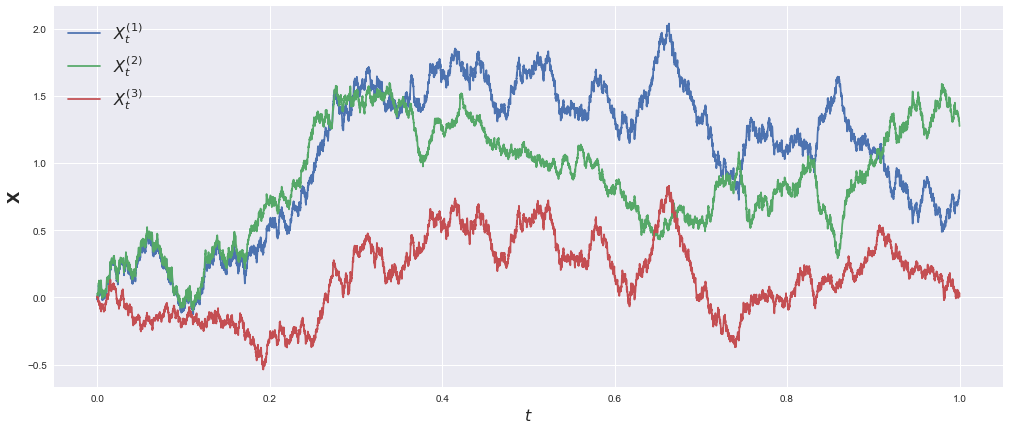
\includegraphics[scale=0.4]{X3}
			\caption{$\mathbf{X}(t)$ from Example \ref{exmp X3}}
			\smallskip
			\small
			One can observe that $X_1(t)$ and $X_2(t)$ have strong positive correlation in the beginning, which decreases over time and later, when $t$ approaches $1$, turns into negative one. Meanwhile $X_3(t)$ has independent fluctuations on the borders, but in the middle it repeats the behavior of $X_1(t)$.
		\end{center}
	\end{figure}
	
	\section{The relation between RCV and ICV}
	
	\begin{defn} \label{stoch calc notions}
		Recall the basic notions from the theory of stochastic calculus (without loss of generality we assume that all the processes have a starting point at $0$ almost surely):
		\begin{enumerate}
			\item An \define{Itô process} $X(t)$ is defined to be an adapted stochastic process that can be expressed as the sum of an integral with respect to time and an integral with respect to Brownian motion:
			\[ X(t) = \int_{0}^{t} \mu(s) ds + \int_{0}^{t} \sigma(s) dW(s). \]
			Here, $\mu(s)$ denotes a (locally bounded) drift process, whereas $\sigma(s)$ is assumed to be a c$\grave{\text{a}}$dl$\grave{\text{a}}$g volatility process.
			\item Let $X$ be a continuous local martingale. Then $[X](t)$ with
			\[ [X](t) = X^2(t) - 2 \int_0^t X(s)dX(s) \]
			is called \define{quadratic variation} of $X$. Note that for deterministic processes quadratic variation is equal to $0$.
			\item The \define{quadratic covariation} of two continuous semimartingales $X$ and $Y$ is defined as follows:
			\[ [X, Y](t) = \frac{1}{4}([X + Y](t) - [X-Y](t)). \]
		\end{enumerate}
	\end{defn}
	
	\begin{lmm} \label{stoch calc notions2} \
		\begin{enumerate}
			\item Let $X$ and $Y$ be Itô processes with volatilities ${\sigma_X}(t)$ and ${\sigma_Y}(t)$ with respect to the same Brownian motion, then
			\[[X](t) = \int_0^t \sigma_X^2(s) ds, \quad [Y](t) = \int_0^t \sigma_Y^2(s) ds \]
			and
			\[ [X, Y](t) = \int_0^t {\sigma_X}(s){\sigma_Y}(s) ds. \]
			\item Quadratic covariation is symmetric and bilinear map:
			\[ [X + Y, Z](t) = [X, Z](t) + [Y, Z](t), \]
			\[ [X, Y + Z](t) = [X, Y](t) + [X, Z](t), \]
			\[ [X, Y](t) = [Y, X](t), \quad [X](t) = [X, X](t). \]
	    \end{enumerate}
	\end{lmm}
	
	\begin{exmp} \label{quad var} \
		\begin{enumerate}
			\item 
			Let us first consider two-dimensional case with $\boldsymbol{\mu}(t) = (\mu_1(t), \mu_2(t))^T$ and
			\[\Theta(t) = \begin{pmatrix}
			\sigma_{11}(t) & \sigma_{12}(t) \\
			\sigma_{21}(t) & \sigma_{22}(t)
			\end{pmatrix} \]
			Then $\mathbf{X}(t) = (X(t), Y(t))^T$, where 
			\[X(t) = \int_0^t\mu_1(s) ds + \int_0^t\sigma_{11}(s) dW_1(s) + \int_0^t\sigma_{12}(s) dW_2(s)\] 
			and
			\[Y(t) = \int_0^t\mu_2(s) ds + \int_0^t\sigma_{21}(s) dW_1(s) + \int_0^t\sigma_{22}(s) dW_2(s).\]
			Using Definition \ref{stoch calc notions} and Lemma \ref{stoch calc notions2} we get
			\[
			[X](t) = \int_{0}^{t}(\sigma_{11}^2(s) +\sigma_{12}^2(s)) ds, \quad  [Y](t) = \int_{0}^{t}(\sigma_{21}^2(s) +\sigma_{22}^2(s)) ds
			\]
			and
			\begin{equation} \label{quadratic variation Ito}
			[X, Y](t) = \int_{0}^{t}(\sigma_{11}(s)\sigma_{21}(s) + \sigma_{12}(s)\sigma_{22}(s)) ds. 
			\end{equation}
			Let us look at the quadratic covariation $[X, Y]$ at time $1$. It is defined as follows: let $\Pi = \{ \tau_0, \dots, \tau_n \}$ be a partition of $[0, 1]$ (i.e. $0 = \tau_0 < \tau_1 < \dots \tau_n = 1$) and set up the sampled cross variation
			\begin{equation} \label{cross variation}
			\sum_{\ell = 1}^{n} \Delta X_\ell \Delta Y_\ell = \sum_{\ell = 1}^{n} (X(\tau_\ell) - X(\tau_{\ell-1})) \cdot (Y(\tau_\ell) - Y(\tau_{\ell-1})).
			\end{equation}
			Now let the number of partition points $n$ go to infinity as the length of the longest subinterval $\| \Pi \| = \max_{1 \leq \ell \leq n}(\tau_{\ell} - \tau_{\ell-1}) $ goes to zero. The sum in \eqref{cross variation} converges in probability to $[X, Y](1)$. This limit is given by the right-hand side of \eqref{quadratic variation Ito}. This assertion follows from the standard theorems in the theory of stochastic calculus. Writing formally,
			\[  \lim_{n \rightarrow \infty} \sum_{\ell = 1}^{n} \Delta X_\ell \Delta Y_\ell \xrightarrow{\mathbb{P}} [X, Y](1). \]
			Hence,
			\[
			\lim_{n \rightarrow \infty} \sum_{\ell=1}^{n}\Delta \mathbf{X}_\ell(\Delta \mathbf{X}_\ell)^T
			= \lim_{n \rightarrow \infty} \sum_{\ell=1}^{n}\begin{pmatrix}
			(\Delta X_\ell)^2 & \Delta X_\ell \Delta Y_\ell \\
			\Delta Y_\ell \Delta X_\ell & (\Delta Y_\ell)^2
			\end{pmatrix} 
			\xrightarrow{\mathbb{P}} 
			\begin{pmatrix}
			[X](1) & [X, Y](1) \\
			[Y, X](1) & [Y](1)
		    \end{pmatrix}.
			\]
			On the other hand,
			\[ \Theta(t) \cdot \Theta^T(t) = \begin{pmatrix}
			\sigma_{11}^2(t) + \sigma_{12}^2(t) & \sigma_{11}(t)\sigma_{21}(t) + \sigma_{12}(t)\sigma_{22}(t) \\
			\sigma_{11}(t)\sigma_{21}(t) + \sigma_{12}(t)\sigma_{22}(t)  & \sigma_{21}^2(t) + \sigma_{22}^2(t)
			\end{pmatrix}. \]
			Taking the integral of $\Theta(t) \cdot \Theta^T(t)$ we conclude that
			\[ \lim_{n \rightarrow \infty} \Sigma_2^{RCV} \xrightarrow{\mathbb{P}} \Sigma_2. \]
			\item 
			The convergence of realized covariance to ICV can be generalized for arbitrary $p$. Let's set $\boldsymbol{\mu}(t) = (\mu_1(t), \dots, \mu_p(t))^T$ and
			\[ 
			\Theta(t) = \begin{pmatrix}
			\Theta_{11}(t) & \dots & \Theta_{1p}(t) \\
			\vdots & \ddots & \vdots \\
			\Theta_{p1}(t) & \dots & \Theta_{pp}(t)
			\end{pmatrix}.
			\]
			Then we have $\mathbf{X}(t) = (X_1(t), \dots, X_p(t))^T$ with
			\[X_j(t) =  \int_0^t\mu_j(s) ds +  \sum_{i=1}^{p} \int_0^t \Theta_{ji}(s) dW_i(s) \]			
			for all $1 \leq j \leq p$. By Definition \ref{stoch calc notions} and Lemma \ref{stoch calc notions2} again
			\[ [X_j](t)= \int_0^t \bigg( \sum_{i=1}^{p} \Theta_{ji}^2(s) \bigg) ds \]
			and
			\[ [X_j, X_k](t) = \int_0^t \bigg(  \sum_{i=1}^{p} \Theta_{ji}(s) \cdot \Theta_{ki}(s) \bigg) ds \]
			for all $1 \leq j,k \leq p$.
			We also have
			\[ 
			\Big(\Theta(t) \cdot \Theta^T(t) \Big)_{jk}   = \sum_{i=1}^{p} \Theta_{ji}(t) \cdot \Theta_{ki}(t).
			\]
			Therefore, we get
			\[  \lim_{n \rightarrow \infty} \sum_{\ell=1}^{n}\Delta \mathbf{X}_\ell(\Delta \mathbf{X}_\ell)^T \xrightarrow{\mathbb{P}} [\mathbf{X}, \mathbf{X}](1), \]
			where 
			\[ \Big( [\mathbf{X}, \mathbf{X}](t)\Big)_{ij} = [X_i, X_j](t), \]
			and finally
			\[ \lim_{n \rightarrow \infty} \Sigma_p^{RCV} \xrightarrow{\mathbb{P}} \Sigma_p. \]
		\end{enumerate}
		
		\begin{rmrk}
			Let ICV matrix $\Sigma_p$ be deterministic. RCV matrix $\Sigma_p^{RCV}$, on the other side, is random by definition. In Example \ref{quad var} we used quadratic covariation as an intermediate step to prove the convergence of one matrix to another. Alternatively to Definition \ref{stoch calc notions} (iii) quadratic covariation can be defined as a limit of the sum of squared random differences, that means, that it is also random. Having almost sure degenerate distribution of quadratic covariation is one of the major properties of Itô processes and it doesn't need to hold for all martingales in general.
		\end{rmrk}
		
	\end{exmp}
	
	\chapter{Marchenko-Pastur law}
	\section{Empirical spectral distribution}
	\begin{rmrk}
		In Example \ref{quad var} we claimed the convergence of RCV matrix to ICV for any finite $p$. In practice, however, it might be the case that the number of processes is approximately equal to the number of observations for each process. Theoretically, the problem arises when the dimension of $p$ has at least the same rate of growth as $n$. In this case the convergence is not well defined, because the RCV matrix has the unlimited size. Then, it is more convenient to study another criteria.
	\end{rmrk}
	
	\begin{defn}
		Let $\mathbf{A}$ be a $p \times p$ Hermitian matrix and $\{\lambda_j:j=1,\dots, p\}$ be a set of its eigenvalues, then
		\[F^{\mathbf{A}}(x) \coloneqq \frac{\#\{j:\lambda_j \leq x\}}{p}, \quad x \in \MR, \]
		where $\#\{ \cdot \}$ denotes the number of elements in the set indicated, is called \define{empirical spectral distribution (ESD)} of $A$.
	\end{defn}
	
	\begin{rmrk}
		A simple fact is that the $h$-th moment of $F^{\mathbf{A}}$ can be written as
		\[ \int x^h dF^{\mathbf{A}}(x) = \frac{\tr(\mathbf{A}^h)}{p}. \]
	\end{rmrk}
	
	\begin{exmp} \label{ESD finite p}
		Take the simplest case with $\boldsymbol{\mu}(t) = 0$ and $\Theta(t) = \gamma(t) \cdot \mathbb{I}_{p \times p}$ with some deterministic process $\gamma(t)$. Let also $\sigma^2 = \int_{0}^{1} \gamma^2(t) dt$, then $\Sigma_p = \sigma^2 \mathbb{I}_{p \times p}$ and its ESD
		\[ F^{\Sigma_p}(x) = 1_{[\sigma^2, \infty)}(x) \]
		is a simple step function. In general case, where $\Sigma_p$ have different eigenvalues, ESD is a combination of such step functions.
	\end{exmp}
	
	\begin{rmrk}
		A naive estimator of the spectral distribution of the ICV matrix $\Sigma_p$ is the spectral distribution of the RCV matrix $\Sigma_p^{RCV}$. In particular, one might wish that the ESD $F^{\Sigma_p^{RCV}}$ of $\Sigma_p^{RCV}$ would approximate $F^{\Sigma_p}$ well when the value of $n$ sufficiently high, namely
		\[ \lim_{n \rightarrow \infty} F^{\Sigma_p^{RCV}} \rightarrow F^{\Sigma_p}. \]
		From the large dimensional random matrix theory (LDRMT) it follows that in the high dimensional setting this good wish won't always come true. For example, in the simplest case when the drift process $\boldsymbol{\mu}(t) \equiv 0$, covolatility process $\Theta(t)$ is constant, and observation times $\tau_\ell$ are equally spaced ($\tau_\ell = \ell / n$), we are in the setting of estimating the usual covariance matrix using the sample covariance matrix, given $n$ i.i.d. $p$-dimensional observations $(\Delta \mathbf{X}_\ell)_{\ell=1, \dots, n}$. From LDRMT, it is well known that if $p/n$ converges to a non-zero number and the ESD $F^{\Sigma_p}$ of the true covariance matrix converges, then the ESD $F^{\Sigma_p^{RCV}}$ of the sample covariance matrix also converges (see e.g. Marchenko and Pastur (1967), Yin(1968), Silverstein and Bai (1995) and Silverstein (1995)). However, the relationship between the limiting spectral distribution (LSD) of $\Sigma_p^{RCV}$ in this case and the LSD of $\Sigma_p$ still can be described, namely by a Marchenko-Pastur equation through Stieltjes transforms.
	\end{rmrk}
	
	\begin{defn}
		In mathematics, the \define{Stieltjes transformation} $m_\mu(z)$ of a measure $\mu$ on $\MR$ is the function of the complex variable $z \in \mathbb{C}_+ \coloneqq \{ z \in \mathbb{C} : \Im(z)>0 \}$ defined by the formula
		\[  
		m_\mu(z) = \int_{t \in \MR} \frac{1}{t - z} d\mu(t).
		\]
		The inversion formula is given by
		\begin{equation} \label{inverse Stieltjes transform}
		\mu([a, b]) + \frac{\mu(\{a\}) + \mu(\{b\})}{2}  = \frac{1}{\pi} \lim_{\eta \rightarrow 0^+} \int_{a}^{b} \Im (m_\mu(z+i\eta)) dz.
		\end{equation}
	\end{defn}
	
	\begin{prps}\label{MP law} \
		\begin{enumerate}
			\item for $p = 1, 2, \dots$ and for $1 \leq \ell \leq n$, $\mathbf{Z}_{\ell}^{(p)} = \big(Z_{j\ell}^{(p)}\big)_{1 \leq j \leq p}$ is a $p$-dimensional vector with $Z_{j\ell}^{(p)}$ i.i.d. with mean 0 and variance 1;
			\item $n = n(p)$ with $y_n \coloneqq p/n \rightarrow y > 0$ as $p \rightarrow \infty$;
			\item $\Sigma_p$ is a (possibly random) nonnegative definite $p \times p$ matrix such that its ESD $F^{\Sigma_p}$ converges a.s. in distribution to a probability distribution $H$ on $[0,\infty)$ as $p \rightarrow \infty$;
			\item $\Sigma_p$ and $\mathbf{Z}_\ell^{(p)}$ are independent.
		\end{enumerate}
		Let $\Sigma_p^{1/2}$ be the (nonnegative) square root matrix of $\Sigma_p$ and 
		\[S_p\coloneqq \frac{1}{n} \sum_{\ell=1}^{n} \Sigma_p^{1/2} \mathbf{Z}_\ell^{(p)}(\mathbf{Z}_\ell^{(p)})^T \Sigma_p^{1/2}.\]
		Then a.s. the ESD of $S_p$ converges in distribution to a probability distribution $F$, which is determined by $H$ in that its Stieltjes transform
		\[ m_F(z)\coloneqq\int_{\lambda \in \MR} \frac{1}{\lambda - z} dF(\lambda) , \quad z \in \mathbb{C}_+ \]
		solves the equation
		\begin{equation} \label{MP eq}
		m_F(z) = \int_{\tau \in \MR} \frac{1}{\tau (1-y(1+zm_F(z))) - z } dH(\tau).
		\end{equation}
	\end{prps}
	\begin{proof}
		 See Theorem 1.1 of Silverstein (1995).
	\end{proof}
	
	\begin{rmrk} \
		\begin{enumerate}
			\item It is easy to see that for ESD $F$ its Stieltjes transform can be found by formula
			\begin{equation} \label{Stieltjes transform eig}
			m_F(z) = \frac{1}{p} \sum_{j=1}^p \frac{1}{\lambda_j - z} = \frac{1}{p} \tr(S_p-z\mathbb{I}_{p \times p})^{-1} .
			\end{equation}
			\item Schematically Proposition \ref{MP law} can be depicted as follows
			\[(F^{\Sigma_p^{RCV}}, F^{\Sigma_p}) \xrightarrow[p,n \rightarrow \infty]{} (F, H).\]
			Our goal is to find $F^{\Sigma_p}$ for sufficiently large $p$. First, we approximate $F$ with $F^{\Sigma_p^{RCV}}$ and calculate $m_F(z)$, using, for example, \eqref{Stieltjes transform eig}. Then we derive $H$ via Marchenko-Pastur equation \eqref{MP eq}, and use it as approximation of $F^{\Sigma_p}$. HOW TO DERIVE H???
			\item Note that if $y \rightarrow 0$ limiting distribution function $F$ of $S_p$ matches limiting distribution function $H$ of $\Sigma_p$. This is the case, when $n$ grows faster than $p$ and as we stated before $\Sigma_p^{RCV}$ converges to $\Sigma_p$.
			\item In the special case when $\Sigma_p = \sigma^2 \mathbb{I}_{p \times p}$, where $\mathbb{I}_{p \times p}$ is the $p \times p$ identity matrix, the LSD $F$ has an analytical expression, which can be derived from the following proposition.
		\end{enumerate}
	\end{rmrk}
	
	\begin{prps} \label{one-dim MP}
		Suppose that $\mathbf{Z}_\ell^{(p)}$'s are as in the Proposition \ref{MP law}, and $\Sigma_p = \sigma^2 \mathbb{I}_{p \times p}$ for some $\sigma^2>0$. Then the LSD $F$ has density
		\[ f(x) = \Big(1-\frac{1}{y}\Big)_+\delta_0(x) + \frac{1}{2 \pi \sigma^2 xy} \sqrt{(b-x)(x-a)} \mathbf{1}_{[a,b]}(x), \]
		where $\delta_0(x)$ is a Dirac delta function and
		\[ a = \sigma^2(1-\sqrt{y})^2 \quad \text{and} \quad b = \sigma^2(1+\sqrt{y})^2. \]
		The LSD $F$ in this proposition is called the Marchenko-Pastur law with ratio index $y$ and scale index $\sigma^2$, and will be denoted by $\mathcal{MP}(y, \sigma^2)$.
	\end{prps}
	\begin{proof}
		See, e.g., Theorem 2.5 in Bai (1999).
	\end{proof}
	\begin{figure}
		\begin{center} \centering
			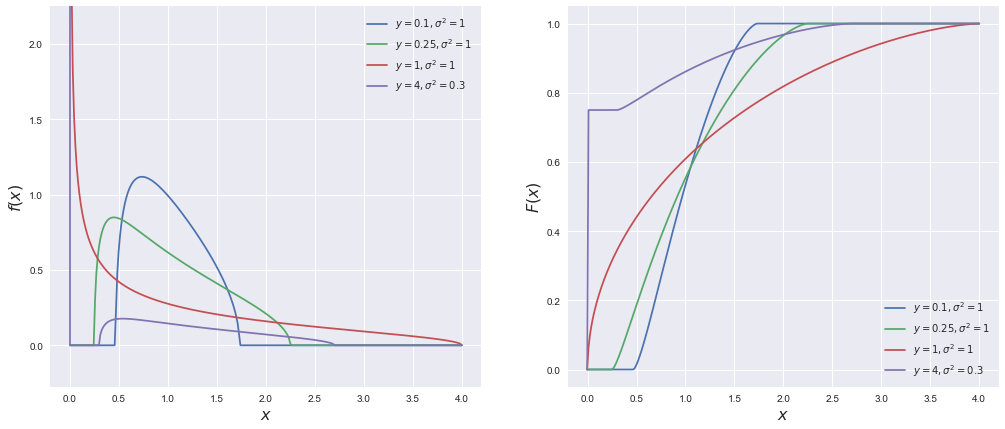
\includegraphics[scale=0.4]{MP}
			\caption{Marchenko-Pastur law}
			\smallskip
			\small
			The left panel shows graphs of the density function $f(x)$ for different parameters $y$ and $\sigma^2$. On the right there are graphs of corresponding cumulative distribution functions $F(x)$. Notice that as $y$ becomes larger the eigenvalues of $\Sigma_p$ spread out instead of concentrating near $\sigma^2$ and the length of the density's support increases.
		\end{center}
	\end{figure}
	
	\begin{rmrk} \
		\begin{enumerate}
			\item We have for $\Sigma_p = \sigma^2 \mathbb{I}_{p \times p}$ the density of limiting spectral distribution
			\[ dH(x) = \delta_{\sigma^2}(x). \]
			Define $m_{\mathcal{MP}}(z)$ as the Stieltjes transform of the Marchenko-Pastur distribution. Then it satisfies the self-consistent equation
			\[
			\begin{aligned}
			m_{\mathcal{MP}}(z) & = \int_{\tau \in \MR} \frac{1}{ \tau( 1-y-zm_{\mathcal{MP}}(z))-z} \delta_{\sigma^2}(x) dx \\
			& =  \frac{1}{ \sigma^2( 1-y-zm_{\mathcal{MP}}(z))-z}.
			\end{aligned}
			\]
			\item Note again that for $y \rightarrow 0$ the density in Proposition \ref{one-dim MP} is
			\[f(x) = \delta_{\sigma^2}(x), \]
			which coincides with the density in Example \ref{ESD finite p} for finite value of $p$ and with density $dH(x)$, because in this case $\Sigma_p^{RCV}$ converges to $\Sigma_p$.
			\item One can show that
			\[ m_{\mathcal{MP}}(z) = \frac{\sigma^2(1-y)-z+ i \sqrt{(b-z)(z-a)}}{2yz}. \]
			Therefore, one can find $m_{\mathcal{MP}}(z)$ through \eqref{Stieltjes transform eig} and derive $\sigma^2$ from it easily.
		\end{enumerate}
		\begin{proof}
			See, e.g., Lemma 2.18 in Ben Adlam
		\end{proof}
	\end{rmrk}
	
	\section{Non-constant volatility case}
	\begin{rmrk}
		In practice, the covolatility process is typically neither constant, nor even deterministic. Furthermore, stock volatility might also depend on the price process itself. Generally, for any time-varying covolatility process $\Theta(t)$, we associate it with a constant covolatility process given by the square root of the ICV matrix
		\[ \Theta^0(t) = \sqrt{\int_0^1\Theta(s) \cdot \Theta^T(s) ds} \quad \forall t \in [0, 1]. \]
		Let $\mathbf{X}^0(t)$ be such that
		\[ d\mathbf{X}^0(t) = \Theta^0(t) d\mathbf{W}(t). \]
		Note that $\mathbf{X}(t)$ and $\mathbf{X}^0(t)$ share the same ICV matrix at time 1:
		\[ \Sigma_p^0 \coloneqq  \int_0^1 \Theta^0(t) \cdot {\Theta^0}^T(t) dt = \int_0^1 dt \int_0^1\Big( \Theta(s) \cdot {\Theta}^T(s)\Big) ds = \Sigma_p.  \]
		Based on $\mathbf{X}^0(t)$, we have an associated RCV matrix
		\[ \Sigma_p^{RCV^0} = \sum_{\ell=1}^{n} \Delta \mathbf{X}_\ell^0 (\Delta \mathbf{X}_\ell^0)^T. \]
		Since $\Sigma_p^{RCV}$ and $\Sigma_p^{RCV^0}$ are based on the same estimation method and share the same targeting ICV matrix, it is desirable that their ESDs have similar properties. In particular, based on the results in LDRMT and the discussion about constant covolatility case, we have the following convergence property for $\Sigma_p^{RCV^0}$: 
		\[ \lim_{p,n \rightarrow \infty} F^{\Sigma_p} = H \quad \Longrightarrow\quad \lim_{p,n \rightarrow \infty} F^{\Sigma_p^{RCV^0}} = F. \]
		Furthermore, their limits are related to each other via the Marchenko-Pastur equation \eqref{MP eq}. The question is: does this property hold for ESD of $\Sigma_p^{RCV}$? Later we will see that even in the most ideal case, when the covolatility process has the form $\Theta(t) =\gamma(t) \mathbb{I}_{p \times p}$ for some deterministic scalar function $\gamma(t)$, such convergence results may \textit{not} hold for $\Sigma_p^{RCV}$. Moreover, the limit of $F^{\Sigma_p^{RCV}}$ (when it exists) changes according to how the covolatility process evolves over time.
	\end{rmrk}
	
	\begin{defn}
		Let $A$, $B$ be two symmetric $p \times p$ matrices. Then we write
		\[ A \succeq B\]
		to denote that $A-B$ is a positive semidefinite matrix. Similarly, we say that $A \preceq B$ if $A-B$ is negative semidefinite. The partial ordering defined by $\succeq$ is called L\"owner ordering.
	\end{defn}
	
	\begin{lmm}[Weyl's Monotonicity Theorem] \label{Weyl}
		Suppose $A$ and $B$ are symmetric, $p \times p$ matrices. Let $\lambda_i(A)$ be the $i$-th largest eigenvalue of $A$. If $A \preceq B$, then $\lambda_i(A) \leq \lambda_i(B)$ for all $i$, or, equivalently
		\[ F^B(x) \leq F^A(x) \quad \forall x \geq 0. \]
    \end{lmm}
    \begin{proof}
    	Corollary 4.3.3 in Horn and Johnson (1990).
    \end{proof}
		
	\begin{prps} \label{counter RCV}
		Suppose that for any $p$, $\mathbf{X}(t)$ is a $p$-dimensional process satisfying
		\begin{equation}
		d \mathbf{X}(t) = \gamma(t) d\mathbf{W}(t), \quad t \in [0, 1],
		\end{equation}
		where $\gamma(t) > 0$ is a nonrandom (scalar) c$\grave{\text{a}}$dl$\grave{\text{a}}$g process. Let $\sigma^2 = \int_0^1 \gamma^2(t) dt$ and so that the ICV matrix $\Sigma_p = \sigma^2 \mathbb{I}_{p \times p}$. Assume further that the observation times $\tau_{\ell}$ are equally spaced, that is, $\tau_{\ell} = \ell / n$, and that the RCV matrix $\Sigma_p^{RCV}$ is defined by \eqref{RCV}. Then so long as $\gamma(t)$ is not constant on $[0, 1)$, for any $\varepsilon > 0$, there exists $y_c = y_c(\gamma, \varepsilon) > 0$ such that if $\lim p/n = y \geq y_c$,
		\begin{equation}
			\limsup F^{\Sigma_p^{RCV}}(b(y)+\sigma^2\varepsilon) < 1 \quad \text{a.s.}
		\end{equation}
		In particular, $F^{\Sigma_p^{RCV}}$ doesn't converge to the Marchenko-Pastur law $\mathcal{MP}(y, \sigma^2)$.
    \end{prps}
    
    \begin{proof}
    	By assumption if $\gamma(t)$ is non-contant, there exists $\delta > 0$ and an interval $[c, d] \subseteq [0, 1] $ such that
    	\[ \gamma(t) \geq \sigma(1+\delta) \quad \forall t \in [c, d]. \]
    	Therefore, if $\big[ \frac{\ell - 1}{n}, \frac{\ell}{n} \big] \subseteq [c, d] $ for some $1 \leq \ell \leq n$, then
    	\[ \Delta \mathbf{X}_\ell (\Delta \mathbf{X}_\ell )^T \stackrel{d}{=} \int_{(\ell-1)/n}^{\ell/n} \gamma^2(t) dt \cdot \mathbf{Z}_\ell(\mathbf{Z}_\ell)^T \succeq \frac{(1+\delta)^2}{n} \sigma^2 \mathbf{Z}_\ell(\mathbf{Z}_\ell)^T,  \]
    	where $\mathbf{Z}_\ell = (Z_{1\ell}, \dots , Z_{p\ell})^T$ consists of independent standard normals. Hence, if we let $ J_n = \big\{ \ell: \big[ \frac{\ell - 1}{n}, \frac{\ell}{n} \big] \subseteq [c, d] \big\} $ and
    	\[ \Gamma_p = \sum_{\ell \in J_n} \Delta \mathbf{X}_\ell (\Delta \mathbf{X}_\ell )^T, \quad \Lambda_p = \frac{\sigma^2}{n(d-c)} \sum_{\ell \in J_n} \mathbf{Z}_\ell (\mathbf{Z}_\ell )^T,  \]
    	then for any $x \geq 0$, by Weyl's Monotonicity Theorem,
    	\[
    	F^{\Sigma_p^{RCV}}(x) \leq F^{\Gamma_p}(x) \leq F^{\Lambda_p}\bigg(\frac{x}{(1+\delta)^2(d-c)}\bigg).
    	\]
	    Now note that $\# J_n \sim (d-c)n$, hence if $p/n \rightarrow y$, by Proposition \ref{MP law}, $F^{\Lambda_p}$ will converge a.s. to the Marchenko-Pastur law with ratio index $y'=\frac{y}{d-c}$ and scale index $\sigma^2$.
	    By the formula of $b(\cdot)$ in Marchenko-Pastur density
	    \[
	    \begin{aligned}
	    (1+\delta)^2(d-c)b(y') &=(1+\delta)\sigma^2 \cdot (1+\delta)(d-c)(1+2\sqrt{y'}+y') \\
	    & =(1+\delta)\sigma^2 \cdot (1+\delta)(d-c + 2\sqrt{(d-c)y} + y) \\
	    & \coloneqq (1+\delta)\sigma^2 \cdot  g(y).
	    \end{aligned}
	    \]
	    Note that the $g(y)$ has a linear growth in $y$ with coefficient $1+\delta$. Hence, for any $\varepsilon > 0$, there exists $y_c > 0$, such that for all $y \geq y_c$
	    \[ g(y) \geq (1+\sqrt{y})^2+\varepsilon,  \]
	    that is,
	    \[ (1+\delta)^2(d-c)b(y') \geq (1+\delta) \sigma^2 \cdot ((1+\sqrt{y})^2+\varepsilon) = (1+\delta)(b(y)+\sigma^2\varepsilon)  \]
	    or, equivalently,
	    \[ \frac{b(y) + \sigma^2\varepsilon}{(1+\delta)^2(d-c)} \leq \frac{b(y')}{1+\delta}. \]
	    Therefore, when the above inequality holds,
	    \[\limsup F^{\Sigma_p^{RCV}}(b(y) + \sigma^2\varepsilon) \leq \limsup F^{\Lambda_p}\bigg(\frac{b(y')}{1+\delta}\bigg) < 1. \]
    \end{proof}
    
    \begin{rmrk}
    	In the proof of Proposition \ref{counter RCV} we saw that more volatility process varies in time, the bigger value of $\delta$ can be found, and hence more the maximum value of domain of $F^{\Sigma_p^{RCV}}$ goes away from $b(y)$. Therefore ESD of $\Sigma_p^{RCV}$ cannot be considered as consistent estimator anymore. In the next part we will study different estimator, which is based on the whole behavior of volatility process.
    \end{rmrk}
    
    \chapter{Non-constant covolatility process}
    
    \section{Limiting distribution for realized covariance}
    \begin{rmrk}
    	In this chapter we will state two major theorems. The first one is a generalization of Proposition \ref{MP law} for limiting spectral distribution of RCV matrix in the case of non-constant covolatility. The second theorem claims the convergence of ESD of alternative estimator to Marchenko-Pastur law. Both theorems require some additional assumptions.
    \end{rmrk}
    
    
    \begin{defn}
    	Suppose that for all $p$ $\mathbf{X}(t) = \mathbf{X}^{(p)}(t)$ is a $p$-dimensional process satisfying \eqref{X diffeq}, and $\Theta(t)$ is c$\grave{\text{a}}$dl$\grave{\text{a}}$g. We say that $\mathbf{X}(t)$ belongs to \define{class $\mathcal{C}$} if, almost surely, there exist $\gamma(t): [0, 1] \mapsto \MR$ and $\Lambda$ a $p \times p$ matrix satisfying $\tr(\Lambda \Lambda^T) = p$ such that 
    	\begin{equation} \label{class C cov}
    	\Theta(t) = \gamma(t) \Lambda.
    	\end{equation}
    	Observe that if \eqref{class C cov} holds, then the ICV matrix $\Sigma_p = \int_{0}^{1} \gamma^2(t) dt \cdot \Lambda \Lambda^T$. The special case when $\Lambda = \mathbb{I}_{p \times p}$ will be studied in simulations.
    \end{defn}
    
    \begin{exmp} \label{exmp C}
    	Suppose that $X_j(t)$ satisfy
    	\[ dX_j(t) = \mu_j(t) dt + \sigma_j(t) dW_j(t), \quad j = 1, \dots, p, \]
    	where $\mu_j(t), \sigma_j(t) : [0, 1] \rightarrow \MR$ are the drift and volatility processes for stock $j$, and $W_j(t)$'s are  (one-dimensional) standard Brownian motions. If the following conditions hold:
    	\begin{itemize}
    		\item the correlation matrix process of $(W_j(t))$
    		\[ R(t)\coloneqq \bigg(\frac{ [W_j, W_k](t) \ }{t}\bigg)_{1 \leq j,k \leq p} =:(r_{jk})_{1 \leq j,k \leq p} \]
    		is constant in $t \in [0, 1]$.
    		\item $r^{(jk)} \neq 0$ for all $1 \leq j,k \leq p$; and
    		\item the correlation matrix process of $X_j(t)$
    		\[ \Bigg( \frac{\int_{0}^{t} \sigma_j(s) \sigma_k(s)  d[W_j, W_k](s) }{\sqrt{\int_{0}^{t} \sigma_j^2(s) ds \cdot \int_{0}^{t} \sigma_k^2(s) ds}} \Bigg)_{1 \leq j,k \leq p}  =:(\rho_{jk})_{1 \leq j,k \leq p}  \]
    		is constant in $t \in [0, 1]$;
    	\end{itemize}
    	then $\mathbf{X}(t)$ belongs to class $\mathcal{C}$.
    	
    	\begin{proof}
    		For any $t \in [0, 1]$: 
    		\[ \rho_{jk} = \frac{r_{jk} \int_{0}^{t} \sigma_j(s) \sigma_k(s) ds }{\sqrt{\int_{0}^{t} \sigma_j^2(s) ds \cdot \int_{0}^{t} \sigma_k^2(s) ds}}, \]
    		therefore
    		\[ \frac{\rho_{jk}}{r_{jk}} = \frac{\int_{0}^{t} \sigma_j(s) \sigma_k(s) ds/t }{\sqrt{\int_{0}^{t} \sigma_j^2(s) ds/t \cdot \int_{0}^{t} \sigma_k^2(s) ds/t}}. \]
    		Letting $t \downarrow 0$, using l'H$\hat{\text{o}}$pital's rule and noting that $\sigma_j(t)$ are c$\grave{\text{a}}$dl$\grave{\text{a}}$g, we observe that
    		\[ \frac{\rho_{jk}}{r_{jk}} = \frac{\sigma_j(0) \sigma_k(0)}{ \sqrt{\sigma_j^2(0) \cdot \sigma_k^2(0) }} = \pm 1. \]
    		Hence, for all $t \in [0, 1]$:
    		\[ \bigg| \int_{0}^{t}\sigma_j(s) \sigma_k(s) ds \bigg| = \sqrt{\int_{0}^{t} \sigma_j^2(s) ds \cdot \int_{0}^{t} \sigma_k^2(s) ds} . \]
    		By Cauchy-Schwartz inequality, this holds only if $\sigma_j(s)$ and $\sigma_k(s)$ are proportional to each other. Therefore, almost surely, there exists a scalar process $\gamma(t) : [0, 1] \rightarrow \MR$ and a $p$-dimensional vector $(\sigma_1, \dots, \sigma_p)^T$, such that
    		\[ (\sigma_1(t), \dots, \sigma_p(t))^T = \gamma(t) \cdot (\sigma_1, \dots, \sigma_p)^T. \]
    		Now we show that $\mathbf{X}(t)$ belongs to class $\mathcal{C}$. In fact one can always find a $p$-dimensional standard Brownian motion $\widetilde{\mathbf{W}}(t)$, such that 
    		\[ \mathbf{W}(t) = R^{1/2}\widetilde{\mathbf{W}}(t), \]
    		where $\mathbf{W} = (W_1(t), \dots, W_p(t))^T$ and $R$ is a correlation matrix of $\mathbf{W}(t)$, which is constant for all $t \in [0, 1]$ by assumption. Hence, writing $\mu(t) = (\mu_1(t), \dots, \mu_p(t))^T$, we have
    		\[ 
    		\begin{aligned}
    		d\mathbf{X}(t) & = \mu(t) dt + \diag(\sigma_1(t), \dots, \sigma_p(t)) d\mathbf{W}(t) \\
    		&  = \mu(t) dt +\gamma(t) \cdot \diag(\sigma_1, \dots, \sigma_p) R^{1/2} d\widetilde{\mathbf{W}}(t).
    		\end{aligned} \]
    	\end{proof}
    \end{exmp}
    
    \begin{rmrk} \
    	\begin{enumerate}
    		\item In particular, if all Brownian motions in Example \ref{exmp C} are independent of each other, then $R(t)$ is an identity matrix $\mathbb{I}_{p \times p}$. Then correlation matrix process of $X_j(t)$ is a diagonal matrix and we need only to require $\rho_{jj}$ to be constant in $t$. 
    		\item The process in Example \ref{exmp X3} doesn't belong to the class $\mathcal{C}$, because its correlation structure varies in time.
    		\item Observe that if a diffusion process $\mathbf{X}(t)$ belongs to class $\mathcal{C}$, the drift process $\boldsymbol{\mu}(t) = 0$, and $\tau_\ell$'s and $\gamma(t)$ are independent of $\mathbf{W}(t)$, then
    		\[ \Delta \mathbf{X}_\ell = \int_{\tau_{\ell-1}}^{\tau_\ell} \gamma(t) \Lambda d\mathbf{W}(t) \stackrel{d}{=} \sqrt{\int_{\tau_{\ell-1}}^{\tau_\ell} \gamma^2(t)dt} \cdot \overline{\Sigma}^{1/2} \cdot \mathbf{Z}_\ell, \]
    		where $ \overline{\Sigma}^{1/2}$ is the nonnegative square root matrix of
    		\[\overline{\Sigma} \coloneqq \Lambda \Lambda^T \]
    		and $\mathbf{Z}_\ell = (Z_{1\ell}, \dots, Z_{p\ell})^T$ consists of independent standard normals. Therefore, the RCV matrix
    		\[ \Sigma_p^{RCV} = \sum_{\ell=1}^{n} \Delta \mathbf{X}_\ell(\Delta \mathbf{X}_\ell)^T \stackrel{d}{=} \sum_{\ell=1}^{n} w_\ell^n \cdot \overline{\Sigma}^{1/2}\mathbf{Z}_\ell (\mathbf{Z}_\ell)^T \overline{\Sigma}^{1/2} \]
    		with 
    		\[w_\ell^n =\int_{\tau_{\ell-1}}^{\tau_\ell} \gamma^2(t)dt.\]
    		This is similar to the $S_p$ in Proposition \ref{MP law}, except that here the weights $w_\ell^n$ may vary in $\ell$, while in Proposition \ref{MP law} the weights are constantly $1/n$.
    	\end{enumerate}
    \end{rmrk}
    
    \begin{rmrk}
    	In order to avoid confusion, we should specify the designations. For any vector $A = (A_1, \dots, A_n)^T$, $\|A\|_2$ denotes its $L^2$-norm, that is
    	\[ \|A\|_2 = \sqrt{\sum_{\ell=1}^n A_\ell^2 }. \]
    	Note that
    	\[ \|A\|_2^2 = A^T A. \]
    	Let $\mathbf{A}$ be $m \times n$ matrix and $\mathbf{A}^* = \overline{\mathbf{A}^T}$ its conjugate transpose. Let also $\lambda_{\max}(\cdot)$ be the operator, taking the largest eigenvalue. Then
    	\[ \|\mathbf{A} \| = \sqrt{\lambda_{\max} (\mathbf{A}^* \mathbf{A}) } \]
    	denotes a spectral norm of $\mathbf{A}$. The value $\lambda_{\max} (\mathbf{A}^* \mathbf{A})$ is also called singular value of the matrix $\mathbf{A}$.
    \end{rmrk}
    
    \begin{prps} \label{prps 6}
    	Suppose that $\mathbb{P}_n$ are real probability measures with Stieltjes transforms $m_n(z)$. Let $K \subseteq \mathbb{C}_+$ be an infinite set with a limit point in $\mathbb{C}_+$. If $\lim_{n \rightarrow \infty} m_n(z) = m(z)$ exists for all $z \in K$, then there exists a probability measure $\MP$ with Stieltjes transform $m(z)$ if and only if
    	\begin{equation} \label{prps 6 eq}
    		\lim_{\upsilon \rightarrow \infty} i\upsilon \cdot m(i \upsilon) = -1,
    	\end{equation}
    	in which case $\MP_n \rightarrow \MP$ in distribution.
    \end{prps}
    \begin{proof}
    	See, e.g., Theorem 2 of Geronimo and Hill (2003).
    \end{proof}
    
    \begin{thm} \label{Thm 1}
    	Assume that all the conditions in Proposition \ref{MP law} are satisfied. Furthermore,
    	\begin{enumerate}
    		\item $Z_{j\ell}^{(p)}$ have finite moments of all orders;
    		\item $H$ has a finite second moment;
    		\item the weights $w_\ell^n$, $1 \leq \ell \leq n$, $n = 1, 2, \dots$, are all positive, and there exists $\kappa < \infty$ such that the rescaled weights $(nw_\ell^n)$ satisfy
    		\[ \max_n \max_{\ell = 1, \dots, n} (nw_\ell^n) \leq \kappa; \]
    		moreover, almost surely, there exists a c$\grave{\text{a}}$dl$\grave{\text{a}}$g function $w(s): [0, 1] \rightarrow \MR_{+}$, such that
    		\[ \lim_n \sum_{1 \leq \ell \leq n} \int_{(\ell-1)/n}^{\ell/n} |n w_\ell^n - w(s)|ds = 0; \]
    		\item there exists a sequence $\eta_p = o(p)$ and a sequence of index sets $\mathcal{I}_p$ satisfying $\mathcal{I}_p \subset \{1, \dots, p\}$ and $\#\mathcal{I}_p \leq \eta_p$ such that for all $n$ and all $\ell$, $w_\ell^n$ may depend on $\mathbf{Z}_\ell^{(p)}$ but only on $\{ Z_{j\ell}^{(p)}: j \in \mathcal{I}_p \}$;
    		\item there exist $C < \infty$ and $\delta < 1/6$ such that for all $p$, $\| \Sigma_p \| \leq Cp^\delta$ a.s.
    	\end{enumerate}
    	Define $S_p = \sum_{\ell=1}^{n} w_\ell^n \cdot \Sigma_p^{1/2} \mathbf{Z}_\ell^{(p)} (\mathbf{Z}_\ell^{(p)})^T\Sigma_p^{1/2} $. Then, almost surely, the ESD of $S_p$ converges in distribution to a probability distribution $F^w$, which is determined by $H$ and $w(s)$ in that its Stiltjes trasform $m_{F^w}(z)$ is given by
    	\begin{equation} \label{Thm 1 eq}
    	    m_{F^w}(z) = -\frac{1}{z} \int_{\tau \in \MR} \frac{1}{\tau M(z) + 1} dH(\tau)
    	\end{equation}
    	where $M(z)$, together with another function $\tilde{m}(z)$, uniquely solve the following equation in $\mathbb{C}_{+} \times \mathbb{C}_{+}$:
    	\[
    	\left \{
    	\begin{array}{l}
    		M(z) = -\frac{1}{z} \int_{\tau \in \MR} \frac{w(s)}{1 + y \tilde{m}(z)w(s)} ds,  \\
    		\tilde{m}(z) =  -\frac{1}{z} \int_{\tau \in \MR} \frac{\tau}{\tau M(z) + 1} dH(\tau).
    	\end{array}
    	\right.
    	\]
    \end{thm}
    \begin{proof}
    	For notational ease, we shall sometimes omit the sub/superscripts $p$ and $n$ in the arguments below: thus, we write $\mathbf{Z}_\ell$ instead of $Z_\ell^{(p)}$, $w_\ell$ instead of $w_\ell^n$, $\Sigma_p$ instead of $\Sigma_p$, $S$ instead of $S_p$, etc. Also, recall that $y_n = p/n$, which converges to $y > 0$. \\
    	By assumption (iv) we may, without loss of generality, assume that the weights $w_\ell$ are independent of $\mathbf{Z}_\ell$'s. This is because, if we let $\widetilde{Z}_\ell$ be the result of replacing $Z_{j \ell}^{(p)}$, $j \in \mathcal{I}_p$, with independent random variables with the same distribution that are also independent of $w_\ell$, and
    	\[ \widetilde{S}\coloneqq \sum_{\ell=1}^{n} w_\ell \cdot \Sigma^{1/2} \widetilde{Z}_\ell (\widetilde{Z}_\ell)^T \Sigma^{1/2}, \]
    	then $\operatorname{rank}(\widetilde{S}-S) \leq 2 \eta_p$, and so by the rank inequality
    	\[ \| F^A - F^B \| \leq \frac{\operatorname{rank}(A-B)}{p} \]
    	for any $A$, $B$ $p \times p$ Hermitian matrices (see, e.g. Lemma 2.2 in Bai (1999)), $\widetilde{S}$ and $S$ must have the same LSD. \\
    	We proceed according to whether $H$ is a delta measure at $0$ or not. If $H$ is a delta measure at $0$, we claim that $F^w$ is also a delta a measure at $0$, and the conclusion of the theorem holds. The reason is as follows. By assumption (iii) 
    	\[ S = \sum_{\ell = 1}^{n} w_\ell \cdot \Sigma^{1/2} \mathbf{Z}_\ell (\mathbf{Z}_\ell)^T \Sigma^{1/2} \leq \frac{\kappa}{n} \sum_{\ell=1}^{n}\Sigma^{1/2} \mathbf{Z}_\ell (\mathbf{Z}_\ell)^T \Sigma^{1/2} \eqqcolon \kappa \overline{S}.   \]
    	Hence, by Lemma \ref{Weyl} again, for any $x \geq 0$
    	\[ F^S(x) \geq F^{\overline{S}}(x/\kappa). \]
    	However, it follows easily from Proposition \ref{MP law} that $F^{\overline{S}}$ converges to the delta measure at $0$, hence so does $F^S$. \\
    	Below we assume that $H$ is not a delta measure at $0$. 
    	We will skip most of the technical details here, but provide main ideas of the proof instead. The major steps are
    	\begin{itemize}
    		\item Define the sequences $(m_n(z))_n$ and $(M_n(z))_n$ in the similar way as $m_{F^w}(z)$ and $M(z)$, but with respect to the realization of $\mathbf{X}(t)$ for some $n$.
    		\item Show the convergence of such sequences to $m(z)$ and $M(z)$.
    		\item Conclude that the limit is unique.
    		\item Using Proposition \ref{prps 6} state the convergence of probability measure.
    	\end{itemize}
    	Starting from the first step we rewrite equation \eqref{Thm 1 eq} as follows:
    	\[ m_{F^w}(z) = \frac{\tr(-zM(z)\Sigma -z\mathbb{I}_{p \times p})^{-1}}{p}. \]
    	Let us define
    	\[ m_n(z) = \frac{\tr(S-z\mathbb{I}_{p \times p})^{-1}}{p} \]
    	and
    	\[ M_n(z) = -\frac{1}{z} \sum_{\ell=1}^{n} \frac{w_\ell}{ 1+w_\ell \mathbf{r}_\ell^T (S_{(\ell)}-z\mathbb{I}_{p \times p})^{-1} \mathbf{r}_\ell},  \]
    	where
    	\[ S_{(\ell)} \coloneqq S - w_\ell \mathbf{r}_\ell \mathbf{r}_\ell^T \]
    	and 
    	\[ \mathbf{r}_\ell \coloneqq \Sigma^{1/2}\mathbf{Z}_\ell. \]
    	The idea is to show the convergence
    	\begin{equation} \label{3.7}
    	     \frac{\tr(-zM_n(z)\Sigma -z\mathbb{I}_{p \times p})^{-1}  }{p} \rightarrow m_n
    	\end{equation}
    	first. Using some lemmas from linear algebra and prior assumptions, we claim that \eqref{3.7} holds. Then we state that if $m_n(z)$ converges to $m(z)$, then
    	\begin{equation} \label{3.22}
    	 M_n(z) \rightarrow M(z) \coloneqq -\frac{1}{z} \int_{0}^{1} \frac{w(s)}{1+y\widetilde{m}(z)w(s) }ds \neq 0, 
    	\end{equation}
    	where $\widetilde{m}(z)$ is the unique solution in $\mathbb{Q}_1 = \{z \in \mathbb{C}: \Re(z) \geq 0, \Im(z) \geq 0\}$ to the following equation:
    	\begin{equation} \label{3.23}
    	\int_{0}^{1} \frac{1}{1 + y \widetilde{m}(z) w(s)} ds = 1 - y (1 + zm(z)).
    	\end{equation}
    	BLA BLA BLA EXPLAIN IT!!!
    	Therefore, by convergence of $F^{\Sigma_p}$ to $H$
    	\[ 
    	\frac{\tr(-zM_n(z)\Sigma -z\mathbb{I}_{p \times p})^{-1}  }{p} \rightarrow -\frac{1}{z} \int_{\tau \in \MR} \frac{1}{\tau M(z) + 1}dH(\tau). \]
    	But \eqref{3.7} implies that
    	\begin{equation} \label{3.27}
    		m(z) = -\frac{1}{z} \int_{\tau \in \MR} \frac{1}{\tau M(z) + 1}dH(\tau). 
    	\end{equation}
    	Observing that $M(z) \neq 0$, $\Re(M(z)) \geq 0$, and $H$ is not a delta measure at $0$, we obtain that $|m(z)| < \frac{1}{|z|}$. Hence $1+zm(z) \neq 0$, and by \eqref{3.23}, $\widetilde{m}(z) \neq 0$. Based on this, we can get another expression for $M(z)$, as follows. By \eqref{3.22} we have
    	\begin{equation} \label{3.28}
    	\begin{aligned}
    	M(z) & = -\frac{1}{z} \int_{0}^{1} \frac{w(s)}{1+y\widetilde{m}(z) w(s)}ds \\
    	& = \frac{1}{z} \cdot \frac{1}{y\widetilde{m}(z)} \cdot \Big( 1 -  \int_{0}^{1} \frac{1}{1+y\widetilde{m}(z) w(s)}ds\Big)  \\
    	& = \frac{1}{z} \cdot \frac{1}{y\widetilde{m}(z)} \cdot ( 1 - (1 - y (1 + z m(z)) ) ) \\
    	& = \frac{1}{z} \cdot \frac{1 + zm(z)}{\widetilde{m}(z)}.
    	\end{aligned}
    	\end{equation}
    	We can derive another formula for $\widetilde{m}(z)$. By \eqref{3.27} and the fact that $H$ is a probability distribution,
    	\[ 1 + zm(z) = 1 - \int_{\tau \in \MR} \frac{1}{\tau M(z) + 1} dH(\tau) = M(z) \int_{\tau \in \MR} \frac{\tau}{\tau M(z) + 1} dH(\tau).  \]
    	Dividing both sides by $-z \widetilde{m}(z) \neq 0$ and using \eqref{3.28} yield
    	\[ M(z) = -\frac{1+zm(z)}{z\widetilde{m}(z)} = -\frac{M(z)}{z\widetilde{m}(z)} \cdot \int_{\tau \in \MR} \frac{\tau}{\tau M(z) + 1} dH(\tau),  \]
    	and since $M(z) \neq 0$,
    	\begin{equation} \label{3.29}
    		\widetilde{m}(z) = -\frac{1}{z} \int_{\tau \in \MR} \frac{\tau}{\tau M(z) + 1} dH(\tau).
    	\end{equation}
    	For the third step we show that for those $z = i \upsilon$ with $\upsilon$ sufficiently large, there is at most one triple
    	\[ (m(z), M(z), \widetilde{m}(z)) \in \mathbb{Q}_1 \times \mathbb{Q}_1 \times \mathbb{Q}_1, \]
    	that solves the equations \eqref{3.22}, \eqref{3.27} and \eqref{3.29}. THAT CAN BE SHOWN HOW???
    	For the fourth step it remains to verify that $\lim_{\upsilon \rightarrow \infty} i \upsilon \cdot m(i \upsilon) = -1$. In fact, using \eqref{3.27} we get that
    	\begin{equation} \label{3.31}
    		i \upsilon \cdot m(i \upsilon)  = -\int_{\tau \in \MR} \frac{1}{ 1+\tau M(i \upsilon) }dH(\tau).
    	\end{equation}
    	Since $\Re(M(i \upsilon)) \geq 0$, 
    	\[ \Big| \frac{1}{1+\tau M(i\upsilon)}\Big|  \leq 1 \quad \forall \tau \geq 0. \]
    	Moreover, by \eqref{3.22} and that $\Re(\widetilde{m}(z)) \geq 0$,
    	\[ M(i \upsilon) \leq \frac{1}{\upsilon} \int_{0}^{1} w(s)ds, \]
    	hence by the dominated convergence theorem, the right-hand side of \eqref{3.31} converges to $-1$ as $\upsilon \rightarrow \infty$.
    \end{proof}
    
    \begin{rmrk}
    	If $w_\ell^n = 1/n$, then $w(s)=1$, and Theorem \ref{Thm 1} reduces to Proposition \ref{MP law}. Moreover, if $w(s)$ is not constant, that is, $w(s) \neq \int_{0}^{1} w(t) dt$ on $[0, 1]$, then except in the trivial case when $H$ is a delta measure at $0$, the LSD $F^w \neq F$, where $F$ is the LSD in Proposition \ref{MP law} determined by $H(\cdot / \int_{0}^{1} w(t) dt)$. The reason is as follows: firstly, for any $w = w(s)$, the family of distributions	$ \{ F^{cw}:c>0  \} $ is a scale family, i.e. for any $x \geq 0$,
    	\[ F^{cw}(x) = F^w(x/c). \]
    	Hence, it is suffices to show that for any positive $w$ such that $w(s) \not\equiv 1 $ on $[0, 1]$ and $ \int_{0}^{1} w(s)ds = 1 $, $F^w \neq F$. In fact, $F^w = F$ if and only if
    	\[ m_{F^w}(z) = m_F(z) \quad \forall z \in \mathbb{C}_+, \]
    	and by the uniqueness of the solution to the equation \eqref{MP eq} this can be true only if
    	\[ M(z) = -\frac{1-y(1 + z m_F(z))}{z}. \]
    	Suppose this is true, then by \eqref{3.28}
    	\[ \frac{1+zm_F(z)}{\widetilde{m}(z)} = 1-y(1 + z m_F(z)) \]
    	or
    	\[ \frac{1}{1+y\widetilde{m}(z)}=\frac{1+zm_F(z)}{\widetilde{m}(z)}.\]
    	By \eqref{3.23}, the last equation implies that
    	\[ \int_{0}^{1} \frac{1}{1 + y \widetilde{m}(z)w(s) }ds = \frac{1}{1+y\widetilde{m}(z)}. \]
    	Since both sides are analytical in $\widetilde{m}(z)$, we get
    	\[ \int_{0}^{1} \frac{1}{1+uw(s)} ds = \frac{1}{1+u}, \quad \forall u \in \mathbb{C} \text{ such that } \Re(u)>0. \]
    	In particular, focusing on $u > 0$, multiplying both sides by $u$, letting $u \rightarrow \infty$ and applying the monotone convergence theorem to the left hand side yield
    	\begin{equation} \label{suppl rmrk eq}
    	    \int_{0}^{1} \frac{1}{w(s)}ds = 1.
    	\end{equation}
    	However, by the Cauchy-Schwarz inequality, since $\int_{0}^{1} w(s)ds = 1$ \eqref{suppl rmrk eq} holds only if $w(s) \equiv 1$ on $[0, 1]$.
    \end{rmrk}
    
    \begin{prps} \label{prps ups}
    	Suppose that for all $p$, $X^{(p)}(t)$ is a $p$-dimensional process in class $\mathcal{C}$ with some drift process $\boldsymbol{\mu}(t) = (\mu_1^{(p)}(t), \dots, \mu_p^{(p)}(t))^T$, covolatility process $\Theta^{(p)}(t) = \gamma^{(p)}(t) \Lambda^{(p)}$ and $p$-dimensional Brownian motion $\mathbf{W}^{(p)}(t) = (W_1^{(p)}(t), \dots, W_t^{(p)}(t) )^T$. Suppose further that:
    	\begin{enumerate}
    		\item there exists $C_0 < \infty$ such that for all $p$ and all $j = 1, \dots, p$, $|\mu_j^{(p)}(t)| \leq C_0$ for all $t \in [0, 1]$ almost surely;
    		\item $\breve{\Sigma}_p = \Lambda^{(p)} ( \Lambda^{(p)})^T $ is (a possibly random) positive semi-definite $p \times p$ matrix such that its ESD $F^{\breve{\Sigma}_p}$ converges almost surely in distribution to a probability distribution $\breve{H}$ on $[0,\infty)$ as $p \rightarrow \infty$; moreover, $\breve{H}$ has a finite second moment;
    		\item there exist $C < \infty$ and $\delta < 1/6$ such that for all $p$, $\|\breve{\Sigma}_p \| \leq Cp^\delta$ almost surely;
    		\item there exits a sequence $\eta_p = o(p)$ and a sequence of index sets $\mathcal{I}_p$ satisfying $\mathcal{I}_p \subset \{1, \dots, p\}$ and $\#\mathcal{I}_p \leq \eta_p$ such that $\gamma^{(p)}(t)$ may depend on $\mathbf{W}^{(p)}(t)$ but only on $\{W_j^{(p)}(t): j \in \mathcal{I}_p\}$; moreover, there exists $C_1 < \infty$ such that for all $p$, $|\gamma^{(p)}(t)| \leq C_1$ for all $t \in [0, 1]$ almost surely; additionally, almost surely, there exists $\gamma(t): [0, 1] \rightarrow \MR$ such that
    		\[ \lim_{p \rightarrow \infty} \int_{0}^{1} |\gamma^{(p)}(t) - \gamma(t) |dt = 0;  \]
    		\item the observation times $\tau_\ell$ are independent of $\mathbf{X}(t)$; moreover, there exists $\kappa < \infty$ such that the observation durations $\Delta \tau_\ell \coloneqq  \tau_\ell - \tau_{\ell-1}$ satisfy
    		\[ \max_{n} \max_{\ell = 1, \dots, n} (n \cdot \Delta \tau_\ell ) \leq \kappa; \]
    		additionally, almost surely, there exists a process $\upsilon(s) : [0, 1] \rightarrow \MR_+$ such that
    		\[ \lim_{n \rightarrow \infty} \tau_{[ns]} = \Upsilon(s) \coloneqq  \int_{0}^{s} \upsilon(r) dr \quad \forall 0 \leq s \leq 1, \]
    		where for any $x$, $[x]$ stands for its integer part.
     	\end{enumerate}
     	Then, as $p \rightarrow \infty$, $F^{\Sigma_p^{RCV}}$ converges almost surely to a probability distribution $F^w$ as specified in Theorem \ref{Thm 1} for
     	\[ w(s) = \gamma^2(\Upsilon(s)) \cdot \upsilon(s). \]
    \end{prps}
    
    \begin{rmrk} \
    	\begin{enumerate}
    		\item In particular, if we have equally spaced observation times, that is $\tau_\ell = \frac{\ell}{n}$ for all $0 \leq \ell \leq n$,
    		then 
    		\[ \upsilon(s) = 1 \quad \text{and} \quad \Upsilon(s) = s.\]
    		Therefore,
    		$w(s) = \gamma^2(s).$
    		\item In the case of constant volatility $\gamma(s) = 1$ we have $w(s) = \upsilon(s)$. Hence, RCV will converge to Marchenko-Pastur law only if observation times are equally spaced.
    		\item Proposition \ref{prps ups} demonstrates explicitly how $\gamma(s)$ and $\tau_\ell$ affect LSD of RCV matrix. If $\gamma(s)$ and hence $w(s)$ are known, then in principle Theorem \ref{Thm 1} can be used to recover $F^{\Sigma_p}$. However, in general $\gamma(s)$ is unknown and estimating the process $\gamma(s)$ can be challenging and will bring in more complication in the inference. Moreover, equations in Theorem \ref{Thm 1} are different from and more complicated than the classical Marchenko-Pastur equation in Proposition \ref{MP law} and in order to recover $F^{\Sigma_p}$, based on these equations, one has to extend existing algorithms, which are defined for equation \eqref{MP eq}. We shall instead propose an alternative estimator, which overcomes these difficulties.
    	\end{enumerate}
    \end{rmrk}
    
    \section{Time-variance adjusted realized covariance}
    		
    \begin{defn}
   		Suppose that a diffusion process $\mathbf{X}(t)$ belongs to class $\mathcal{C}$. We define \define{time-variation adjusted realized covariance (TVARCV) matrix} as follows:
   		\begin{equation} \label{TVARCV}
   		\widehat{\Sigma}_p \coloneqq \frac{\tr \big( \Sigma_p^{RCV} \big) }{n} \sum_{\ell = 1}^{n} \frac{\Delta \mathbf{X}_\ell (\Delta \mathbf{X}_\ell)^T}{\| \Delta \mathbf{X}_\ell \|_2^2} = \frac{\tr \big( \Sigma_p^{RCV} \big) }{p} \widetilde{\Sigma}_p,
   		\end{equation}
   		where
   		\begin{equation} \label{Sigma_tilde}
   		\widetilde{\Sigma}_p \coloneqq \frac{p}{n} \sum_{\ell = 1}^{n} \frac{\Delta \mathbf{X}_\ell (\Delta \mathbf{X}_\ell)^T}{\| \Delta \mathbf{X}_\ell \|_2^2}.
   		\end{equation}
    \end{defn}
    
    \begin{rmrk}
    	Let us explain $\widetilde{\Sigma}_p$. Consider the simplest case when $\mu(t) = 0$, $\gamma(t)$ is deterministic, $\Lambda_t = \mathbb{I}_{p \times p}$, and $\tau_{\ell} = \ell / n$, $\ell = 0, 1, \dots, n$. In this case,
    	\[ \Delta \mathbf{X}_\ell = \sqrt{\int_{(\ell - 1)/n}^{\ell / n} \gamma^2(t) dt }\cdot \frac{\mathbf{Z}_\ell}{\sqrt{n}}, \]
    	where $\mathbf{Z}_\ell = (Z_{1\ell}, \dots, Z_{p\ell})^T$ is a vector of i.i.d. standard normal random variables. Hence,
    	\[ \frac{\Delta \mathbf{X}_\ell (\Delta \mathbf{X}_\ell)^T}{\| \Delta \mathbf{X}_\ell \|_2^2} = \frac{\mathbf{Z}_\ell \mathbf{Z}_\ell^T}{\|  \mathbf{Z}_\ell \|_2^2}. \]
    	However, as $p \rightarrow \infty$, $\| \mathbf{Z}_\ell \|_2^2 \sim p$, hence
    	\[ \widetilde{\Sigma}_p \sim \frac{\sum_{\ell = 1}^{n}\mathbf{Z}_\ell \mathbf{Z}_\ell^T}{n}, \]
    	the latter being the usual sample covariance matrix.
    	We will show that, first, $\tr(\Sigma_p^{RCV}) \sim \tr(\Sigma_p)$; and second, if $\mathbf{X}(t)$ belongs to class $\mathcal{C}$ and satisfies certain additional assumptions, then the LSD of $\widetilde{\Sigma}_p$ is related to that of $\breve{\Sigma}_p$ via the Marchenko-Pastur equation, where
    	\[ \breve{\Sigma}_p = \frac{p}{\tr(\Sigma_p)}\Sigma_p = \Lambda \Lambda^T. \]
    	Hence, the LSD of $\widehat{\Sigma}_p$ is also related to that of $\Sigma_p$ via the same Marchenko-Pastur equation.
    	We will now state our assumptions for the major theorem in this paper.
    \end{rmrk}
    
    \begin{asmp} \label{asmp2} \
    	\begin{enumerate}
    		\item there exists $C_0 < \infty$ such that for all $p$ and all $j = 1, \dots, p$, $|\mu_j^{(p)}(t)| \leq C_0$ for all $t \in [0, 1]$ a.s.;
    		\item there exist constants $C_1 < \infty$, $0 \leq \delta_1 < 1/2$, a sequence $\eta_p < C_1 p^{\delta_1}$ and a sequence of index sets $\mathcal{I}_p$ satisfying $\mathcal{I}_p \subset \{ 1, \dots p \}$ and $\# \mathcal{I}_p \leq \eta_p$ such that $\gamma^{(p)}(t)$ may depend on $\mathbf{W}^{(p)}(t)$ but only on $\{ W_j^{(p)}(t) : j \in \mathcal{I}_p \}$; moreover, there exists $C_2 < \infty$ such that for all $p$, $|\gamma^{(p)}(t)| \in (1/C_2, C_2)$ for all $t \in [0, 1]$ a.s.;
    		\item there exists $C_3 < \infty$ such that for all $p$ and for all $j$, the individual volatilities \[ \sigma_j(t) = \gamma^{(p)}(t)\sqrt{\sum_{k=1}^{p} (\Lambda_{jk}^{(p)})^2} \in (1/C_3, C_3)\] for all $t \in [0, 1]$ a.s.;
    		\item \[ \lim_{p \rightarrow \infty} \frac{\tr(\Sigma_p)}{p} = \lim_{p \rightarrow \infty} \int_{0}^{1} (\gamma^{(p)}(t))^2 dt \coloneqq \theta > 0 \quad \text{a.s.}; \]
    		\item almost surely, as $p \rightarrow \infty$, the ESD $F^{\Sigma_p}$ converges to a probability distribution $H$ on $[0, \infty)$;
    		\item there exist $C_5 < \infty$ and $0 \leq \delta_2 < 1/2$ such that for all $p$, $\| \Sigma_p \| \leq C_5 p^{\delta_2}$ a.s.;
    		\item the $\delta_1$ in (ii) and $\delta_2$ in (vi) satisfy that $\delta_1 + \delta_2 < 1/2$;
    		\item $p/n \rightarrow y \in (0, \infty) $ as $p \rightarrow \infty$; and
    		\item there exists $C_4 < \infty$ such that for all $n$,
    		\[ \max_{1 \leq \ell \leq n} n \cdot (\tau_{\ell} - \tau_{\ell - 1}) \leq C_4 \quad \text{a.s.}  \]
    		moreover, $\tau_{\ell}$'s are independent of $\mathbf{X}(t)$.
    	\end{enumerate}
    \end{asmp}
    
    \begin{lmm}[Burkholder-Davis-Gundy inequality] \label{BDG}
    	For any real number $p \geq 1$ there exist positive constants $c_p$ and $C_p$ such that, for all local martingales $X(t)$ with $X(0) = 0$, its maximum processes $M(t) = \sup_{t \leq s} |X(s)|$ and stopping times $\tau$, the following inequalities hold
    	\[ c_p \ME[[X]^{p/2}(\tau)] \leq \ME[M^p(\tau)] \leq C_p \ME[[X]^{p/2}(\tau)]. \]
    \end{lmm}
    \begin{proof}
    	See, e.g., Revuz and Yor (1998).
    \end{proof}
    
    \begin{defn}
    	Let $F$ and $G$ be two cumulative distribution functions. Then the \define{L$\acute{\text{e}}$vy distance} between them is
    	\[ L(F, G) \coloneqq \inf \{ \varepsilon > 0 : F(x-\varepsilon) -\varepsilon \leq G(x) \leq F(x+\varepsilon) + \varepsilon \quad \forall x\in\MR   \} \]
    \end{defn}
    
    \begin{lmm} \label{lmm1}
    	Suppose that for each $p$, $\mathbf{v}_\ell^{(p)} = (v_{1\ell}^{(p)}, \dots, v_{p\ell}^{(p)})^T$ and $\mathbf{w}_\ell^{(p)} = (w_{1\ell}^{(p)}, \dots, w_{p\ell}^{(p)})^T$, $\ell = 1, \dots, n$, are all $p$-dimensional vectors. Define
    	\[	\widetilde{S}_n = \sum_{\ell = 1}^{n} (\mathbf{v}_\ell^{(p)} + \mathbf{w}_\ell^{(p)}) \cdot (\mathbf{v}_\ell^{(p)} + \mathbf{w}_\ell^{(p)})^T\]
    	and
    	\[S_n = \sum_{\ell = 1}^{n} \mathbf{w}_\ell^{(p)} (\mathbf{w}_\ell^{(p)})^T. \]
    	If the following conditions are satisfied:
    	\begin{enumerate}
    		\item $\lim_{p \rightarrow \infty} p/n = y > 0$;
    		\item there exists a sequence $\varepsilon_p = o(1/\sqrt{p})$ such that for all $p$ and all $\ell$, all the entries of $\mathbf{v}_\ell^{(p)}$ are bounded by $\varepsilon_p$ in absolute value;
    		\item $ \limsup_{p \rightarrow \infty} {\tr(S_n)}/{p} < \infty$ almost surely.
    	\end{enumerate}
    	Then $L(F^{\widetilde{S}_n}, F^{S_n}) \rightarrow 0$ almost surely.
    \end{lmm}
    \begin{proof}
    	For notational ease we shall omit the superscript $p$ and write $\mathbf{v}_\ell = \mathbf{v}_\ell^{(p)}$, $\mathbf{w}_\ell = \mathbf{w}_\ell^{(p)}$, $v_{j\ell} = v_{j\ell}^{(p)}$, etc. For each $p$ set 
    	\[ \mathbf{A} = \mathbf{A}_p = (\mathbf{v}_1 + \mathbf{w}_1, \dots, \mathbf{v}_n + \mathbf{w}_1) \]
    	and
    	\[ \mathbf{B} = \mathbf{B}_p = (\mathbf{w}_1, \dots,  \mathbf{w}_n). \]
    	Then
    	\[ \widetilde{S}_n = \mathbf{AA}^T \quad \text{and} \quad S_n = \mathbf{BB}^T. \]
    	By Lemma 2.7 of Bai (1999)
    	\[L^4(F^{\widetilde{S}_n}, F^{S_n}) \leq \frac{2}{p^2} \tr((A-B)(A-B)^T) \cdot \tr(\widetilde{S}_n + S_n). \]
    	By condition (ii),
    	\[ \tr((\mathbf{A}-\mathbf{B})(\mathbf{A}-\mathbf{B})^T)  = \sum_{\ell=1}^{n} \sum_{j=1}^{p} v_{j\ell}^2 \leq np \cdot \varepsilon_p^2. \]
    	Moreover,
    	\[
    	\begin{aligned}
    	\tr(\widetilde{S}_n) &= \sum_{\ell=1}^{n} \sum_{j=1}^{p} (v_{j\ell} + w_{j\ell})^2 \\
    	& \leq 2 \sum_{\ell=1}^{n} \sum_{j=1}^{p} v_{j\ell}^2 + 2\sum_{\ell=1}^{n} \sum_{j=1}^{p} w_{j\ell}^2 \\
    	& \leq 2np \cdot \varepsilon_p^2 + 2 \tr(S_n).
    	\end{aligned}
    	 \]
    	 Therefore,
    	 \[L^4(F^{\widetilde{S}_n}, F^{S_n}) \leq 4n^2\varepsilon_p^4 + 6n\varepsilon_p^2 \frac{\tr(S_n)}{p}. \]
    	 The conclusion follows since $\varepsilon_p = o(1/\sqrt{p})$ and hence $o(1/\sqrt{n})$.
    \end{proof}
    
    \begin{lmm} \label{lmm 9}
    	For $\mathbf{X} = (X_1, \dots, X_p)^T$, where $X_j$'s are i.i.d. random variables such that $\ME[X_1] = 0$, $\Var(X_1) = 1$ and $\ME[|X_1|^{2k}] < \infty$ for some $2 \leq k \in \MN$, there exists $C_k \geq 0$, depending only on $k$, $\ME[|X_1|^4]$ and $\ME[|X_1|^{2k}]$, such that for any $p \times p$ nonrandom matrix $\mathbf{A}$,
    	\[ \ME[|\mathbf{X}^* \mathbf{A} \mathbf{X} - \tr(\mathbf{A}) |^{2k}] \leq C_k(\tr(\mathbf{AA}^*))^k \leq C_k p^k \|\mathbf{A} \|^{2k}  \]
    \end{lmm}
    \begin{proof}
    	See, e.g., Lemma 2.7 of Bai and Silverstein (1998).
    \end{proof}
    
    \begin{lmm} \label{trace conv}
    	Under Assumptions \ref{asmp2} (iv), namely, suppose that
    	\[ \lim_{p \rightarrow \infty} \frac{\tr(\Sigma_p)}{p} = \theta \quad \text{a.s.}, \]
    	then
    	\[ \lim_{p \rightarrow \infty} \frac{\tr(\Sigma_p^{RCV})}{p} = \theta \quad \text{a.s.} \]
    \end{lmm}
    \begin{proof}
    	The full proof can be found in supplementary article OF THE PAPER .... We will provide here the main idea: it suffices to show that
    	\[ \frac{\tr(\Sigma_p^{RCV})-\tr(\Sigma_p)}{p} \xrightarrow[p \rightarrow \infty]{} 0 \quad \text{a.s.} \]
    	Let us first consider one-dimensional process
    	\[ dX(t) = \mu(t)dt + \sigma(t)dW(t). \]
    	Under slight assumptions it can be shown that there exist constants $c$, $C_1$ and $C_2$, such that for all $0 \leq x \leq c \sqrt{n}$
    	\[\MP\Big(\sqrt{n} \Big| [X, X](1) - \int_{0}^{1} \sigma^2(t)dt \Big| \geq x \Big) \leq C_1 \exp \{ -C_2 x^2 \}. \]
    	Therefore, generalizing it for $p$-dimensional processes, we have for every $1 \leq j \leq p$
    	\[ \MP(\sqrt{n} |(\Sigma_p^{RCV})_{jj} - (\Sigma_p)_{jj} | > x) \leq C_1 \exp \{ -C_2 x^2 \}. \]
    	Hence, for any $0 < \varepsilon < c$ and for all $p$,
    	\[ 
    	\begin{aligned}
    	\MP \Bigg(  \Bigg| \frac{\tr(\Sigma_p^{RCV})-\tr(\Sigma_p)}{p}  \Bigg| \geq \varepsilon \Bigg) & \leq \sum_{j=1}^{p} \MP(\sqrt{n} |(\Sigma_p^{RCV})_{jj} - (\Sigma_p)_{jj} | \geq \varepsilon) \\
    	& \leq p \cdot C_1 \exp \{ -C_2 \varepsilon^2 \cdot n  \}.
    	\end{aligned}
    	\]
    	The almost sure convergence then follows from the Borel-Cantelli lemma\footnote{
    		Let $X_1, X_2, \dots$ be a sequence of random variables in some probability space and $\varepsilon > 0$ be arbitrary.
    		Then
    		\[ \sum_{n=1}^{\infty} \MP(|X_n| \geq \varepsilon) < \infty \Longrightarrow X_n \xrightarrow{a.s.} 0.  \]
    	}.
    \end{proof}
    
    \begin{crlr} \label{crlr trace conv}
    	The main results of the Lemma \ref{trace conv} are the convergence of $\breve{\Sigma}_p$ 
    	\[ \lim_{p \rightarrow \infty} \breve{\Sigma}_p \rightarrow \frac{1}{\theta} \Sigma_p \]
    	and of TVARCV estimator
    	\[ \lim_{p \rightarrow \infty} \widehat{\Sigma}_p \rightarrow \theta \widetilde{\Sigma}_p. \]
    \end{crlr}
    
    \begin{rmrk} \label{Thm 2 expl}
    	Using Lemma \ref{trace conv} we state that ESD of $\breve{\Sigma}_p$ converges almost surely:
    	\[\lim_{p,n \rightarrow \infty} F^{\breve{\Sigma}_p} \rightarrow \breve{H} \quad \text{a.s.},\] 
    	where $\breve{H}$ is defined by
    	\[\breve{H}(x) = H(\theta x) \quad \forall x \geq 0. \]
    	It is obvious, since
    	\[ F^{\breve{\Sigma}_p} = F^{\Sigma_p}(\tr(\Sigma_p)/p \cdot x) \quad \forall x \geq 0. \]
    	Now it is left to prove the following:
    	\[\lim_{p,n \rightarrow \infty}   F^{\widetilde{\Sigma}_p} \rightarrow \widetilde{F} \quad \text{a.s.}, \]
    	where the LSD $\widetilde{F}$ of $\widetilde{\Sigma}_p$ is determined by $\breve{H}$ in that its Stieltjes transform $m_{\widetilde{F}}(z)$ satisfies the equation
    	\[ m_{\widetilde{F}}(z) = \int_{\tau \in \MR} \frac{1}{ \tau(1- y(1 + zm_{\widetilde{F}}(z))) - z } d\breve{H}(\tau). \]
    	Then the convergence of $\widehat{\Sigma}_p$ will follow from the Corollary \ref{crlr trace conv}.
    \end{rmrk}
    
    \begin{thm} \label{Thm 2}
    	Suppose that for all $p$, $\mathbf{X}(t) = \mathbf{X}^{(p)}(t)$ is a $p$-dimensional process in class $\mathcal{C}$ for some drift process $\boldsymbol{\mu}^{(p)}(t) = (\mu_1^{(p)}(t), \dots , \mu_p^{(p)}(t))^T$, covolatility process $\Theta^{(p)}(t) = \gamma^{(p)}(t) \Lambda^{(p)}$ and a $p$-dimensional Brownian motion $\mathbf{W}_t^{(p)}$, which satisfy Assumptions \ref{asmp2} (i)-(vii) above. Suppose also that $p$ and $n$ satisfy Assumptions \ref{asmp2} (viii), and the observation times satisfy Assumptions \ref{asmp2} (ix). Let $\hat{\Sigma}_p$ be as in \eqref{TVARCV}. Then, as $p \rightarrow \infty$, $F^{\hat{\Sigma}_p}$ converges a.s. to a probability distribution $F$, which is determined by $H$ through Stieltjes transforms via the same Marchenko-Pastur equation as in Proposition \ref{MP law}.
    \end{thm}
    \begin{proof}
    	We only need to show the convergence of $F^{\widetilde{\Sigma}_p}$. For notational ease, we shall omit the superscript $p$ in the arguments below: thus we write $\boldsymbol{\mu}(t)$ instead of $\boldsymbol{\mu}^{(p)}(t)$, $\gamma(t)$ instead of $\gamma^{(p)}(t)$, $\Lambda$ instead of $\Lambda^{(p)}$, etc. First, note that
    	\[ \Delta \mathbf{X}_\ell = \int_{\tau_{\ell-1}}^{\tau_\ell} \boldsymbol{\mu}(t) dt + \Lambda \cdot \int_{\tau_{\ell-1}}^{\tau_\ell} \gamma(t) d\mathbf{W}(t) \coloneqq \sqrt{\int_{\tau_{\ell-1}}^{\tau_\ell} \gamma^2(t) dt}\cdot (\mathbf{v}_\ell + \Lambda \cdot \mathbf{Z}_\ell), \]
    	where
    	\[ \mathbf{v}_\ell = (v_{1\ell}, \dots, v_{p\ell})^T = \frac{\int_{\tau_{\ell-1}}^{\tau_\ell} \boldsymbol{\mu}(t) dt}{\sqrt{\int_{\tau_{\ell-1}}^{\tau_\ell} \gamma^2(t) dt}} \]
    	and
    	\[ \mathbf{Z}_\ell = (Z_{1\ell}, \dots, Z_{p\ell})^T = \frac{\int_{\tau_{\ell-1}}^{\tau_\ell} \gamma(t) d\mathbf{W}(t)}{\sqrt{\int_{\tau_{\ell-1}}^{\tau_\ell} \gamma^2(t) dt}} \]
    	By performing an orthogonal transformation if necessary, without loss of generality, we may assume that the index set $\mathcal{I}_p \subset \{ 1, \dots, \eta_p \} $. Then by Assumptions \ref{asmp2} (ii) and (ix), for $j > \eta_p$, $Z_{j\ell}$ are i.i.d. $\sim \mathcal{N}(0, 1)$. Write
    	\[ \mathbf{U}_\ell = (Z_{1\ell}, \dots Z_{\eta_p\ell})^T \]
    	and 
    	\[ \mathbf{D}_\ell = (Z_{\eta_{p}+1\ell}, \dots Z_{p\ell})^T.\]
    	With the above notation, $\widetilde{\Sigma}_p$ can be rewritten as
    	\begin{equation}
    	\widetilde{\Sigma}_p = y_n \sum_{\ell=1}^{n} \frac{\Delta \mathbf{X}_\ell (\Delta \mathbf{X}_\ell)^T}{\|\Delta \mathbf{X}_\ell\|_2^2} = y_n \sum_{\ell=1}^{n} \frac{(\mathbf{v}_\ell + \Lambda \mathbf{Z}_\ell) (\mathbf{v}_\ell + \Lambda \mathbf{Z}_\ell)^T}{\|\mathbf{v}_\ell + \Lambda \mathbf{Z}_\ell\|_2^2}
    	\end{equation}
    	By Assumptions \ref{asmp2} (i), (ii) and (ix), there exists $C > 0$, such that $|v_{j\ell}| \leq C / \sqrt{n}$ for all $j$ and $\ell$, hence $\| \mathbf{v}_\ell\|_2$'s are uniformly bounded. We will show that
    	\begin{equation} \label{334}
    		\max_{\ell = 1, \dots, n} \Bigg|\frac{  \| \Lambda \mathbf{Z}_\ell \|_2^2}{p} - 1\Bigg| = \max_{\ell = 1, \dots, n} \Bigg| \frac{  \mathbf{Z}_\ell^T \breve{\Sigma}_p \mathbf{Z}_\ell}{p} - 1\Bigg| \rightarrow 0 \quad \text{a.s.},
    	\end{equation}
    	which clearly implies that
    	\begin{equation} \label{335}
    		\max_{\ell = 1, \dots, n} \Bigg|\frac{  \| \mathbf{v}_\ell + \Lambda\mathbf{Z}_\ell  \|_2^2}{p} - 1\Bigg| \rightarrow 0 \quad \text{a.s.}
    	\end{equation}
    	To prove \eqref{334} let us write
    	\[ \breve{\Sigma}_p = \begin{pmatrix}
    	\mathbf{A} & \mathbf{B} \\
    	\mathbf{B}^T & \mathbf{C}
    	\end{pmatrix}, \]
    	where $\mathbf{A}$, $\mathbf{B}$ and $\mathbf{C}$ are $\eta_p \times \eta_p$, $\eta_p \times (n - \eta_p)$ and $(n-\eta_p) \times (n-\eta_p)$ matrices, respectively. Then
    	\[ \mathbf{Z}_\ell^T \breve{\Sigma}_p \mathbf{Z}_\ell = \mathbf{U}_\ell^T \mathbf{A} \mathbf{U}_\ell + 2\mathbf{D}_\ell^T \mathbf{B}^T \mathbf{U}_\ell + \mathbf{D}_\ell^T \mathbf{C} \mathbf{D}_\ell.  \]    	
    	By a well-known fact about the spectral norm,
    	\[ \|\mathbf{A}\| \leq \|\breve{\Sigma}_p \|, \quad \|\mathbf{B}\| \leq \|\breve{\Sigma}_p \| \quad \text{and} \quad \|\mathbf{C}\| \leq \|\breve{\Sigma}_p \|. \]
    	In particular, by Assumptions \ref{asmp2} (ii), (vi) and (vii),
    	\[ 0 \leq \tr(\mathbf{A}) \leq \eta_p \cdot \|\breve{\Sigma}_p \| \leq Cp^{\delta_1 + \delta_2} = o(p), \]
    	hence 
    	\[ \frac{\tr(\mathbf{C})}{p} = \frac{\tr(\breve{\Sigma}_p)-\tr(\mathbf{A})}{p} \rightarrow 1. \]
    	Now using the fact that $\mathbf{D}_\ell$ consists of i.i.d. standard normals, Assumptions \ref{asmp2} and Lemma \ref{lmm 9} we get for any $k \in \MN$
    	\[ \ME[ |\mathbf{D}_\ell^T \mathbf{C} \mathbf{D}_\ell - \tr(\mathbf{C})|^{2k}] \leq C_k p^k \cdot C_5 p^{2 \delta k} = C_k' p^{(2\delta+1)k}.  \]
        Using Markov's inequality\footnote{
        	Markov's inequality states that for any non-negative random variable $X$, $k \in \MN$ and $n \in \MR_+$ the following inequality holds:
        	\[ \MP(X \geq n) \leq \frac{\ME[X^k]}{n^k}. \]
        } we get that for any $\varepsilon > 0$,
        \[ \MP(|\mathbf{D}_\ell^T \mathbf{C} \mathbf{D}_\ell - \tr(\mathbf{C})| \geq p\varepsilon ) \leq \frac{C_k' p^{(2\delta+1)k}}{p^{2k}\varepsilon^{2k}} = C_k' p^{(2\delta-1)k}\varepsilon^{-2k} \quad \forall 1 \leq \ell \leq n. \]
        Hence, choosing $k > \frac{2}{1-2\delta}$, using Borel-Cantelli and that $n = O(p)$ yield
    	\[ \max_{\ell = 1, \dots, n} \Bigg| \frac{\mathbf{D}_\ell^T \mathbf{C} \mathbf{D}_\ell}{p} - 1 \Bigg| \rightarrow 0 \quad \text{a.s.} \]
    	To complete the proof of \eqref{334}, it then suffices to show that
    	\[ \max_{\ell = 1, \dots, n} \frac{| \mathbf{U}_\ell^T \mathbf{A} \mathbf{U}_\ell |}{p} \rightarrow 0 \quad \text{and} \quad \max_{\ell = 1, \dots, n} \frac{| \mathbf{D}_\ell^T \mathbf{B} \mathbf{U}_\ell |}{p} \rightarrow 0 \quad \text{a.s.} \]
    	We shall only prove the first convergence, the second one can be proved similarly. We have
    	\begin{equation} \label{337}
    		|\mathbf{U}_\ell \mathbf{A} \mathbf{U}_\ell| \leq \|\mathbf{A}\| \cdot \|\mathbf{U}_\ell\|_2^2 \leq C_5 p^{\delta_2} \cdot \|\mathbf{U}_\ell\|_2^2
    	\end{equation}
    	Observe that for all $1 \leq i \leq \eta_p$, by Assumptions \ref{asmp2} (ii),
    	\[ | Z_\ell^{(i)} |^2 = \frac{|\int_{\tau_{\ell-1}}^{\tau_\ell} \gamma_t d\mathbf{W}_t|^2}{\int_{\tau_{\ell-1}}^{\tau_\ell} \gamma_t^2 dt} \leq \frac{C_2^2}{\tau_\ell-\tau_{\ell-1} } \cdot \Bigg|\int_{\tau_{\ell-1}}^{\tau_\ell} \gamma_t d\mathbf{W}_t \Bigg|^2. \] 
    	By Lemma \ref{BDG} , we then get that for any $k \in \MN$, there exists $\lambda_k > 0$ such that
    	\begin{equation} \label{338}
    		\ME[ |Z_\ell^{(i)}|^{2k} ] \leq \lambda_k C_2^{4k}.
    	\end{equation}
    	Now we are ready to show that $\max_{\ell = 1, \dots, n} \frac{| \mathbf{U}_\ell^T \mathbf{A} \mathbf{U}_\ell |}{p} \rightarrow 0 $. In fact, for any $\varepsilon > 0$, for any $k \in \MN$, by Markov's inequality, \eqref{337}, H\"older's inequality and \eqref{338},
    	\[ 
    	\begin{aligned}
    	\MP(\max_{\ell = 1, \dots, n} | \mathbf{U}_\ell^T \mathbf{A} \mathbf{U}_\ell | \geq p\varepsilon) & \leq \sum_{\ell=1}^{n} \MP(|\mathbf{U}_\ell^T \mathbf{A} \mathbf{U}_\ell | \geq p\varepsilon) \\
    	& \leq \sum_{\ell=1}^{n} \frac{\ME[ |\mathbf{U}_\ell^T \mathbf{A} \mathbf{U}_\ell|^k ]}{ p^k \varepsilon^k } \\
    	& \leq \sum_{\ell=1}^{n} \frac{ C_5^k p^{k \delta_2}  \cdot \eta_p \cdot \lambda_k C_2^{4k} \cdot \eta_p^{k-1} }{p^k\varepsilon^k} \\
    	& \leq C p^{1+k\delta_2 + k\delta_1 - k}.
    	\end{aligned}
    	 \]
    	 By Assumptions \ref{asmp2} (vii), $\delta_1 + \delta_2 < 1/2$, hence by choosing $k$ to be large enough, the right hand side will be summable in $p$: 
    	 \[ \sum_{p=1}^{\infty} \MP\big(\max_{\ell = 1, \dots, n} | \mathbf{U}_\ell^T \mathbf{A} \mathbf{U}_\ell | \geq p\varepsilon\big) < \infty. \]
    	 Hence by Borel–Cantelli lemma, almost surely, $\max_{\ell = 1, \dots, n} \frac{| \mathbf{U}_\ell^T \mathbf{A} \mathbf{U}_\ell |}{p} \rightarrow 0$.
    	 We now get back to $\widetilde{\Sigma}_p$. By \eqref{335}, for any $\varepsilon > 0$, almost surely, for all $n$ sufficiently large, for all $\ell = 1, \dots, n$,
    	 \[ p(1-\varepsilon) \leq \| \mathbf{v}_\ell + \Lambda \mathbf{Z}_\ell \|_2^2 \leq p(1+\varepsilon). \]
    	 Hence, almost surely, for all $n$ sufficiently large,
    	 \[ \frac{1}{1+\varepsilon} \widetilde{S}_p \preceq \widetilde{\Sigma}_p = y_n \sum_{\ell=1}^{n} \frac{(\mathbf{v}_\ell + \Lambda \mathbf{Z}_\ell) (\mathbf{v}_\ell + \Lambda \mathbf{Z}_\ell)^T}{\|\mathbf{v}_\ell + \Lambda \mathbf{Z}_\ell\|_2^2} \preceq \frac{1}{1-\varepsilon} \widetilde{S}_p, \]
    	 where
    	 \[  \widetilde{S}_p = \frac{1}{n}\sum_{\ell=1}^{n} (\mathbf{v}_\ell + \Lambda \mathbf{Z}_\ell) (\mathbf{v}_\ell + \Lambda \mathbf{Z}_\ell)^T. \]
    	 Hence, by Weyl's Monotonicity theorem,
    	 \begin{equation} \label{339}
    	     F^{\widetilde{S}_p}((1+\varepsilon)x) \geq F^{\widetilde{\Sigma}_p}(x) \geq F^{\widetilde{S}_p}((1-\varepsilon)x) \quad \forall x \geq 0.
    	 \end{equation}
    	 Next, by Lemma \ref{lmm1} $\widetilde{S}_p$ has the same LSD as 
    	 \[S_p \coloneqq \frac{1}{n} \sum_{\ell=1}^{n} \Lambda \mathbf{Z}_\ell (\mathbf{Z}_\ell)^T \Lambda^T.\]
    	 Moreover, by using the same trick as in the beginning of the proof of Theorem \ref{Thm 1}, $F^{S_p}$ has the same limit as $F^{S'_p}$, where
    	 \[S'_p \coloneqq \frac{1}{n} \sum_{\ell=1}^{n} \Lambda \widetilde{\mathbf{Z}}_\ell (\widetilde{\mathbf{Z}}_\ell)^T \Lambda^T\]
    	 and $\widetilde{\mathbf{Z}}_\ell$ consists of i.i.d. standard normals. For $F^{S'_p}$, it follows easily from Proposition \ref{MP law} that it converges to $\widetilde{F}$, because $\breve{\Sigma}_p = \Lambda \Lambda^T$. Moreover, by Theorems 1.1 and 2.1 in Silverstein and Choi (1995), $\widetilde{F}$ is differentiable and in particular continuous at all $x > 0$. It follows from \eqref{339} that $F^{\widetilde{\Sigma}_p}$ must also converge to $\widetilde{F}$.
    \end{proof}
    
    
    \chapter{Stochastic volatility case}
    \begin{rmrk}
    	Stochastic volatility models describe the behavior of volatility of a log-price $\mathbf{X}(t)$ by a function of some auxiliary (possibly multi-dimensional) stochastic process. In this part we give definitions of the models which are the most widely used in a quantitative sphere.
    \end{rmrk}
    
    \begin{defn} \
    	\begin{enumerate}
    		\item 
    		Let $\overline{W}(t)$, $t \geq 0$ be a standard Brownian motion. The \define{Vasicek model} for stochastic process is defined by the stochastic differential equation (SDE)
    		\begin{equation} \label{Vasicek}
    		dZ(t) = \beta(\alpha - Z(t))dt + \xi \overline{W}(t),
    		\end{equation}
    		where $\alpha$, $\beta$ and $\xi$ are positive constants. The solution can be determined in closed form and is
    		\[ Z(t) = Z(0) e^{-\beta t} + \alpha (1 - e^{-\beta t}) + \xi e^{-\beta t} \int_{0}^{t} e^{\beta s}d\overline{W}(s).\]
    		The properties of $Z(t)$ are the following:
    		\begin{itemize}
    			\item $Z(t)$ is normally distributed with mean
    			\[ \ME[Z(t)] = e^{-\beta t} Z(0) + \alpha(1-e^{-\beta t}) \]
    			and variance
    			\[ \Var(Z(t)) = \frac{\xi^2}{2\beta} (1-e^{-2\beta t}). \]
    			\item The model is mean-reverting with long-run mean $\alpha$. That means, $Z(t)$ tends to reach $\alpha$, and once it does it, it starts to fluctuate near its vicinity. Parameter $\beta$ represents the speed of mean reversion and $\xi$ is a parameter, which determines the volatility of the variance process.
    			\item There is a probability that $Z(t)$ will go below zero:
    			\[ \MP(Z(t) < 0) > 0. \]
    		\end{itemize}
    		Due to the last property it is not always convenient to consider this process for volatility modeling.
    		\item
    		The stochastic process $Y(t)$ is called \define{Cox-Ingersoll-Ross (CIR) process}, if it is determined by the following SDE:
    		\begin{equation} \label{CIR}
    		dY(t) = \beta(\alpha - Y(t))dt + \xi\sqrt{Y(t)}d \overline{W}(t),
    		\end{equation}
    		where $\alpha$, $\beta$ and $\xi$ are positive constants, and $\overline{W}(t)$ is a standard Brownian motion. Conditional on parameters, time $t$ and initial value $Y(0)$, scaled CIR process has a non-central chi-squared distribution with $k$ degrees of freedom and non-centrality parameter $\lambda$:
    		\[ c Y(t) \sim {\chi'}_k^2(\lambda),  \]
    		where
    		\[k = \frac{4\alpha \beta}{\xi^2},\ \lambda = Y(0) c e^{-\beta t} \ \text{and} \ c = \frac{4 \beta}{\xi^2 (1-e^{-\beta t})}.\]
    		CIR process never goes below $0$. Moreover, it is a.s. positive if the condition
    		\[ 2\alpha \beta \geq \xi^2  \]
    		is met. This property makes CIR process a perfect tool for volatility (or interest rate) modeling. Also, $Y(t)$ has the same expectation as in Vasicek model, and its variance is
    		\[ \Var(Y(t)) = \frac{\xi^2}{\beta} Y(0) (e^{-\beta t} - e^{-2\beta t}) + \frac{\alpha \xi^2}{2\beta}(1-2e^{-\beta t} + e^{-2\beta t}). \]
    		
    		\item The standard \define{Heston model} assumes that one-dimensional log-price process $X_t$ is determined by the following SDE:
    		\begin{equation}
    		dX(t) = \mu dt + \sqrt{Y(t)}d{W}(t),
    		\end{equation}
    		where $Y(t)$ satisfies SDE \eqref{CIR} and ${W}(t)$ is another standard Brownian motion, such that 
    		\begin{equation} \label{dependent Brownian}
    		[{W}, \overline{W}](t) = \int_{0}^{t}\rho(s) ds
    		\end{equation}
    		holds with a (stochastic) process $\rho(t)$, taking values strictly between $-1$ and $1$. Sometimes equality \eqref{dependent Brownian} is informally written as
    		\[ d{W}(t)\cdot d\overline{W}(t) = \rho(t) dt. \]
    	\end{enumerate}
    \end{defn}
    
    \begin{rmrk}
    	If we are in a Heston model with $\rho(t) \equiv 0$, then we have a closed-form solution for $X(t)$:
    	\[ X(t) \sim \mathcal{N}(\mu t, Y(t) \cdot t ), \]
    	where $Y(t)$ is an independent CIR process and therefore conditionally on $t$ and other parameters has a scaled non-central chi-squared distribution. In the case of nonzero correlation between $Y(t)$ and $X(t)$ one can simulate $X(t)$, using, for example, either Euler discretization, or the exact simulation algorithm (see, e.g., Broadie and Kaya (2004)).
    \end{rmrk}
    
    
    \chapter{Jump-diffusion processes}
    \begin{rmrk}
    	(CHECK TEXT HERE!)
    	Before we discussed pure diffusion processes, namely that these processes are continuous almost sure. In this part we study so-called jump-diffusion processes.
    	It doesn't matter how volatile or random is $\gamma(t)$, until it finite, the process $\mathbf{X}(t)$ will be continuous. In practice, things are different.
    	 It is quite useful to consider so-called jump-diffusion processes... How should we change our estimator then?
    	ALSO MENTION ONE- AND FINITE-DIMENSIONAL PROCESSES, THEN GO FOR P->INF
    	ALSO WE ONLY CONSIDER EQUIDISTANT TIMES
    	AND ONLY SIGMA EQUAL TO IDENTITY, WHICH MEANS INDPENENCE
    	AND MU = 0
    \end{rmrk}
    
    \begin{exmp} \label{uniform jumps} \
    		Simplest model: let $U \sim \mathcal{U}[0, 1]$ be standard uniformly distributed random variable and
    		\begin{equation}
    		d\mathbf{X}(t) = \Theta(t)  d\mathbf{W}(t) + a\Delta_U(t)dt,
    		\end{equation}
    		where $a$ is some positive constant and $\Delta_U(t) = (\delta_U(t), \dots, \delta_U(t))^T$ is a vector of Dirac delta functions shifted to $U$. In other words, all the components of $\mathbf{X}(t)$ make a jump of size $a$ at the same random time $t = U$. Let us denote by $\mathbf{X^c}(t)$ the continuous part of $\mathbf{X}(t)$:
    		\[ d\mathbf{X^c}(t) = \Theta(t) d\mathbf{W}(t). \]
    		Moreover, assume that we have equidistant observation times $\tau_{\ell} = \ell / n$ and let $\ell'$ be the index of interval, where $U$ is located:
    		\[ U \in \bigg[\frac{\ell'-1}{n}, \frac{\ell'}{n}\bigg). \]
    		Then
    		\[ 
    		\begin{aligned}
    		\Sigma_p^{RCV} & = \sum_{\ell=1, \ell \neq \ell'}^{n}\Delta \mathbf{X}_\ell(\Delta \mathbf{X}_\ell)^T + \Delta \mathbf{X}_{\ell'}(\Delta \mathbf{X}_{\ell'})^T\\
    		& = \sum_{\ell=1, \ell \neq \ell'}^{n}\Delta \mathbf{X}_\ell(\Delta \mathbf{X}_\ell)^T + (\Delta \mathbf{X^c}_{\ell'} + a\mathbb{U}_{p \times 1})(\Delta \mathbf{X^c}_{\ell'} + a\mathbb{U}_{p \times 1})^T\\
    		& =  \sum_{\ell=1}^{n}\Delta \mathbf{X^c}_\ell(\Delta \mathbf{X^c}_\ell)^T + a\Delta \mathbf{X^c}_{\ell'} \cdot \mathbb{U}_{1 \times p} + a(\Delta \mathbf{X^c}_{\ell'} \cdot \mathbb{U}_{1 \times p})^T + a^2\mathbb{U}_{p \times p} ,
    		\end{aligned}
    		\]
    		where $\mathbb{U}_{k \times j}$ stands for $k \times j$ matrix filled with ones. Note that the elements of $\Delta \mathbf{X^c}_{\ell'} \cdot \mathbb{U}_{1 \times p}$ are i.i.d. $ \sim \mathcal{N}\big(0, \Gamma_{\ell'}/n )$ with $\Gamma_{\ell'}=\int_{(\ell' - 1)/n}^{\ell' / n} \gamma^2(t) dt$. Therefore, if we set $n \rightarrow \infty$, $\tr(\Sigma_p^{RCV})$ will converge to the same value as before plus $a^2p$. Also,
    		\[
    		\| \Delta \mathbf{X}_{\ell'} \|_2^2 = \| \Delta \mathbf{X^c}_{\ell'} + a\mathbb{U}_{p \times 1} \|_2^2  = \sum_{j=1}^{p} (\Delta X^c_{\ell'})^2 + 2a\sum_{j=1}^{p} \Delta X^c_{\ell'} + a^2p.
    		\]
    		We have asymptotically:
    		\[
    		\sum_{j=1}^{p} (\Delta X^c_{\ell'})^2 \sim \frac{p}{n}\Gamma_{\ell'}
    		\]
    		as a sum of $p$ i.i.d. normally distributed random variables with variance $\Gamma_{\ell'}/n$ and
    		\[ \sum_{j=1}^{p} \Delta X^c_{\ell'} \sim \mathcal{N}\Big(0, \frac{p}{n}\Gamma_{\ell'}\Big). \]
    		As long as $p/n$ converges to some finite constant, $\Gamma_{\ell'}$ is bounded and $p$ converges to infinity, we have
    		\[ 
    		\frac{\Delta \mathbf{X}_{\ell'}(\Delta \mathbf{X}_{\ell'})^T}{\| \Delta \mathbf{X}_{\ell'} \|_2^2} \rightarrow 0.
    		\]
    		Hence, if we know that all components jumped at the same time and the size of the jump is equal to $a$, new estimator will be
    		\[ 
    		\widehat{\Sigma}'_p = \frac{\tr(\Sigma_p^{RCV}) - a^2p}{n} \sum_{\ell=1}^{n} \frac{\Delta \mathbf{X}_{\ell}(\Delta \mathbf{X}_{\ell})^T}{\| \Delta \mathbf{X}_{\ell} \|_2^2}.
    		\]
    \end{exmp}
    
    \begin{rmrk}
    	In Example \ref{uniform jumps} we assumed that in the interval $[0, 1]$ each component of the process $\mathbf{X}(t)$ had exactly one jump and exactly at the same time. In practice, jump-diffusion processes are often modeled using Poisson processes, where one cannot be sure how many jumps and when can happen in given interval.
    \end{rmrk}
    
    \begin{defn} \
    	\begin{enumerate}
    		\item To construct a Poisson process, we begin with a sequence of arrival times $\tau_1^N, \tau_2^N, \dots$, where
    		\[ \tau_{j+1}^N - \tau_j^N \sim \operatorname{Exp}(\lambda) \quad \forall j \geq 1.  \]
    		Value $\tau_j^N$ defines the time of $j$-th jump. \define{The Poisson process} $N(t)$ counts the number of jumps that occur at or before time $t$. More precisely,
    		\[ N(t) = \sum_{j \geq 1} \mathbf{1}_{[\tau_j^N, \infty)} (t). \]
    		Because the expected time between jumps is $1/\lambda$, the jumps are arriving at an average rate of $\lambda$ per unit time. We say the Poisson process $N(t)$ has intensity $\lambda$. The bigger $\lambda$ we have, the larger is the expected amount of jumps.
    		\item Let $N(t)$ be a Poisson process with intensity $\lambda$, and let $Y_1, Y_2, \dots$ be a sequence of i.i.d. random variables with mean
    		\[ \beta = \ME[Y_1]. \]
    		We assume the random variables $Y_1, Y_2, \dots$ are also independent of $N(t)$. We define the \define{compound Poisson process}
    		\[ Q(t) = \sum_{i=1}^{N(t)} Y_i, \quad t \geq 0. \]
    		The jumps in $Q(t)$ occur at the same times as the jumps in $N(t)$, but whereas the jumps in $N(t)$ are always of size $1$, the $j$-th jump in $Q(t)$ is of random size $Y_j$.
    		\item
    		Let $J(t)$ be an adapted, right-continuous \define{pure jump process} with $J(0) = 0$. By right-continuous we mean that $J(t) = \lim_{s \downarrow t}J(s)$ for all $t \geq 0$. In other words, if $J$ has a jump at time $t$, then $J(t)$ is the value of $J$ immediately.  A Poisson process and compound Poisson processes are the examples of pure jump processes. A process $X(t)$ of the form
    		\[ X(t) = \int_{0}^t \mu(s)ds + \int_{0}^{t} \sigma(s) dW(s) + J(t), \]
    		where $\mu(s), \sigma(s)$ are adapted processes and $W(s)$ is a standard Brownian motion is called a \define{jump-diffusion process}.
    	\end{enumerate}
    \end{defn}
    
    \begin{prps}
    	Let $X_1(t) = \int_{0}^t \mu_1(s)ds + \int_{0}^{t} \sigma_1(s) dW(s) + J_1(t)$ be a jump-diffusion process. Then
    	\[ [X_1, X_1](t) = \int_0^t \sigma_1^2(s)ds + \sum_{0 < s \leq t} (\Delta J_1(s) )^2. \]
    	Let also $X_2(t) = \int_{0}^t \mu_2(s)ds + \int_{0}^{t} \sigma_2(s) dW(s) + J_2(t)$, then
    	\[ [X_1, X_2](t) = \int_0^t \sigma_1(s) \sigma_2(s) ds + \sum_{0 < s \leq t} \Delta J_1(s)\Delta J_2(s). \]
    \end{prps}
    \begin{proof}
    	See Theorem 11.4.7 in Shreve
    \end{proof}
    
    \begin{rmrk}
    	Let us again look at the case with fixed $p$. In Example \ref{uniform jumps} we have
    	\[J_j(t) = a\mathbf{1}_{[U, 1]}(t) \quad \forall 1 \leq j \leq p \]
    	and
    	\[ \Sigma_p^{RCV} \xrightarrow{\MP} \Sigma_p + a^2\mathbb{U}_{p \times p}.  \]    	
    	Let us consider the process, determined by the following SDE:
    	\[ dX_j(t) = \sigma dW_j(t) + \Delta N_j(t) \quad \forall 1 \leq j \leq p, \]
    	where $N_j(t)$ are independent Poisson processes. The probability that two jumps happen simultaneously is equal to $0$, hence
    	\[ [X_i, X_j](t) = \sigma^2 \quad \forall 1 \leq i \neq j \leq p. \]
    	Recall that the size of the jumps of Poisson process is equal to $1$ and therefore,
    	\[ \Sigma_p^{RCV} \xrightarrow{\MP} \Sigma_p + \Sigma_p^N\]
    	with
    	\[
    	 \Sigma_p^N \coloneqq \begin{pmatrix}
    	\sum_{i \geq 1} \mathbf{1}_{[0, 1]} (\tau_i^{N_1}) & \cdots & 0 \\
    	\vdots & \ddots & \vdots \\
    	0 & \cdots & \sum_{i \geq 1} \mathbf{1}_{[0, 1]} (\tau_i^{N_p})
    	\end{pmatrix}
    	. \]
    	The limit of $\Sigma_p^{RCV}$ is no longer deterministic, because diagonal elements of $\Sigma_p^N$ are random. \\
    	If one replaces $N_j(t)$ with $Q_j(t)$, then the randomness will only increase.
    	BUT WHAT IF P IS INFINITE?
    \end{rmrk}
    
    \chapter{Simulation studies}
    
    \begin{rmrk}
    	BLA BLA BLA Here we do simulations
    \end{rmrk}
    
    \begin{exmp} \label{SimCos}
    	Let's take an example from the paper... Assume we have equidistant observation times $\tau_{\ell} = \ell / n$, $\boldsymbol{\mu}(t) \equiv 0$ and
    	\[
    	\gamma(t) = \sqrt{0.0009 + 0.0008 \cos(2 \pi t)}.
    	\]
    	Then
    	\[ \sigma^2 = 0.0009 + \int_{0}^{1}0.0008 \cos(2 \pi t) dt = 0.0009. \]
    	Note that
    	\[ \Delta X_{jl} = X_j(\ell/n) - X_j((\ell-1)/n) \sim \mathcal{N}(0, \Gamma_\ell / n ), \]
    	for all $1 \leq j \leq p$, where
    	\[ \Gamma_\ell = \int_{(\ell-1)/n}^{\ell / n} \gamma^2(t)dt = 0.0009 + 0.0008 \cdot \frac{ \sin(2\pi \ell / n )-\sin(2\pi (\ell-1) / n ) }{2\pi}. \]
    	The simulations show that TVARCV estimator converges asymptotically to Marchenko-Pastur law, while RCV doesn't. \\
    	Firstly, we are in a setting $y = 4$. Then $a = 1$ and $b = 9$. The process $\mathbf{X}(t)$, LSD histograms and plot of the density of Marchenko-Pastur law are shown on Figure 6.1. \\
    	In the second case, we run simulations for $y = 1$. Then $a = 0$ and $b = 4$. We will compare it with the next setting.
    \end{exmp}
    
    \begin{figure}[ht]
    	\begin{center} \centering
    		\includegraphics[scale=0.4]{XCos2}
    		\caption{ $\mathbf{X}(t)$ from Example \ref{SimCos}, $n = 1000$, $p=4000$, $\sigma^2 = 0.0009$ }
    		\smallskip
    		\small
    		In this setting $y = p/n = 4$. One the left panel one sees four thousands independent stochastic processes. On the right blue histogram shows ESD of $\Sigma_p^{RCV}$, green histogram -- ESD of $\widehat{\Sigma}_p$ and red curve -- Marchenko-Pastur law. Note point mass equal to $0.75$ at the origin.
    	\end{center}
    \end{figure}
    
    \begin{exmp} \label{PosTimes}
    	Let us set time points $ \{\tau_\ell\}_{0 \leq \ell \leq n}$, where $\tau_0 = 0$ a.s. and interarrival times are independent and obey the exponential distribution with rate $\lambda$, that is 
    	\[ \MP(\tau_{\ell} - \tau_{\ell-1} > x) =  e^{-\lambda x}, \quad 1 \leq \ell \leq n. \]
    	Then by Strong Law of Large Numbers
    	\[ \frac{\tau_n}{n} = \frac{1}{n} \sum_{\ell=1}^{n} (\tau_{\ell} - \tau_{\ell-1}) \xrightarrow{a.s.} \ME[\tau_1] = \lambda. \]
    	Define
    	\[ \mathcal{T} = \{\tau_\ell : \tau_\ell \in [0, 1]\}, \]
    	then by setting $\lambda = \frac{1}{n}$, we get $\#\mathcal{T} \sim n$.
    	Let's take volatility $\gamma_t$ as in Example \ref{SimCos}. Then we have 
    	\[ \Delta X_{jl} = X_j(\tau_\ell) - X_j(\tau_{\ell-1}) \sim \mathcal{N}(0, \Gamma_\ell \cdot (\tau_\ell - \tau_{\ell-1})), \]
    	for all $1 \leq j \leq p$, with
    	\[ \Gamma_\ell = \int_{\tau_{\ell-1}}^{\tau_\ell} \gamma^2(t)dt = 0.0009 + 0.0008\cdot \frac{ \sin(2\pi \tau_\ell )-\sin(2\pi \tau_{\ell-1} ) }{2\pi}. \]
    	According to Proposition \ref{prps ups} different intervals between observation times will affect RCV as strong as fluctuating volatility, and we observe it on the Figure 6.3.
    \end{exmp}
    
    \begin{figure}
    	\begin{center} \centering
    		\includegraphics[scale=0.4]{XCos}
    		\caption{ $\mathbf{X}(t)$ from Example \ref{SimCos}, $n = 1000$, $p=1000$ }
    		\smallskip
    		\small
    		In this setting $y = p/n = 1$. Note, that the domain of $F^{RCV}$ is larger than the domain of Marchenko-Pastur law, as it was proved in Proposition \ref{counter RCV}.
    	\end{center}
    	\begin{center} \centering
    		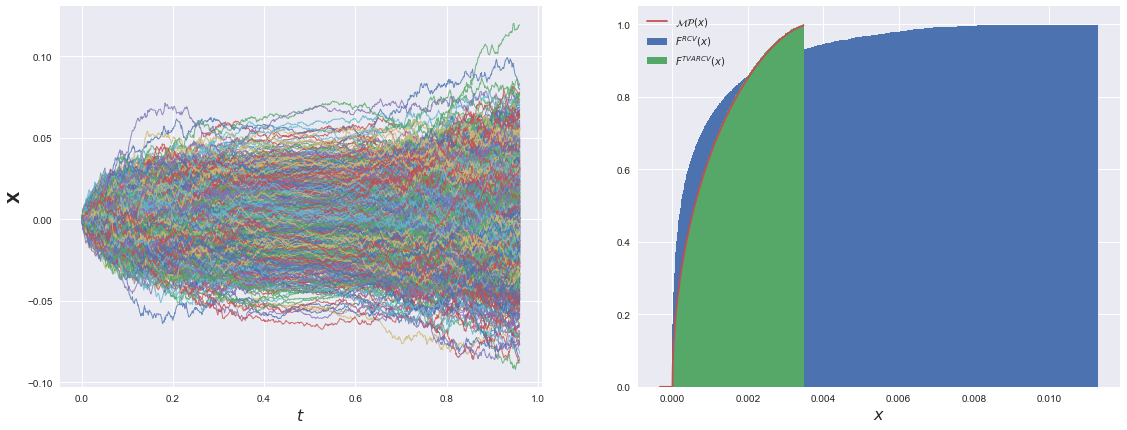
\includegraphics[scale=0.4]{Xcostimes}
    		\caption{ $\mathbf{X}(t)$ from Example \ref{PosTimes}, $n \simeq 1000$, $p=1000$ }
    		\smallskip
    		\small
    		We see that if observation times are not equidistant, the ESD of RCV changes drastically, even if visually there is no difference for paths of $\mathbf{X}(t)$ and volatility process $\gamma(t)$ stays the same.
    	\end{center}
    \end{figure}
    
    \begin{exmp} \label{SimCIR}
    	Let's assume
    	\[ \gamma(t) = \sqrt{Y(t)}, \]
    	where $Y_t$ is a CIR process, determined by \eqref{CIR}. Then it is easy to see that
    	\[ \sigma^2 = \beta\alpha - \beta\int_{0}^{1} \gamma^2(t)dt + \xi \int_{0}^{1} \gamma(t) d\overline{W}(t).\]
    	Therefore, as long as $\xi > 0$, the value of $\sigma^2$ is random and for different realizations of $\gamma_t$ we have different LSD.
    	Moreover, let
    	\[ \overline{W}(t) = \frac{1}{\sqrt{\eta_p}} \sum_{j=1}^{\eta_p}W_j(t), \]
    	where $\eta_p$ is determined by Assumption \ref{asmp2} (ii). The process $\overline{W}(t)$ is still the standard Brownian motion, because it is a.s. continuous, has independent increments and
    	\[ \overline{W}(t) - \overline{W}(s) = \frac{1}{\sqrt{\eta_p}} \sum_{j=1}^{\eta_p}(W_j(t)-W_j(s)) \sim \mathcal{N}(0, t-s) \quad \forall t < s. \]
    \end{exmp}
    
    \begin{rmrk}
    	Theorem \ref{Thm 2} states that as long $\eta_p = o(p)$, TVARCV will converge to Marchenko-Pastur law. But let us take $\eta_p = p$, that means that $\overline{W}(t)$ is a sample average of $\mathbf{W}(t)$ and depends on every of its component $W_j(t)$. Simulations show that even in this case, when Assumptions \ref{asmp2} (ii) are not satisfied, Theorem \ref{Thm 2} still holds and ESD of $\widehat{\Sigma}_p$ converges to Marchenko-Pastur law. Intuitively it can be explained in the following way: \\
    	For any $1 \leq i \leq p$ we have
    	\[ dW_i(t) \cdot d\overline{W}(t) = dW_i(t) \cdot \frac{1}{\sqrt{\eta_p}} \sum_{j=1}^{\eta_p}dW_j(t) = \frac{dt}{\sqrt{\eta_p}} \mathbf{1}_{\{i \leq \eta_p\}}, \]
    	or equivalently 
    	\[ [W_i, \overline{W}](t) =  \frac{t}{\sqrt{\eta_p}} \mathbf{1}_{\{i \leq \eta_p\}} \leq \frac{1}{\sqrt{\eta_p}} .  \]
    	Hence, with growing $\eta_p$ $\overline{W}_t$ is based on bigger amount of components of $\mathbf{W}(t)$, but the dependence becomes smaller and for $\eta_p = p \rightarrow \infty$ correlation between $\overline{W}_t$ and any component of $\mathbf{W}(t)$ goes to $0$.
    \end{rmrk}
    
    \begin{figure}[ht]
    	\begin{center} \centering
    		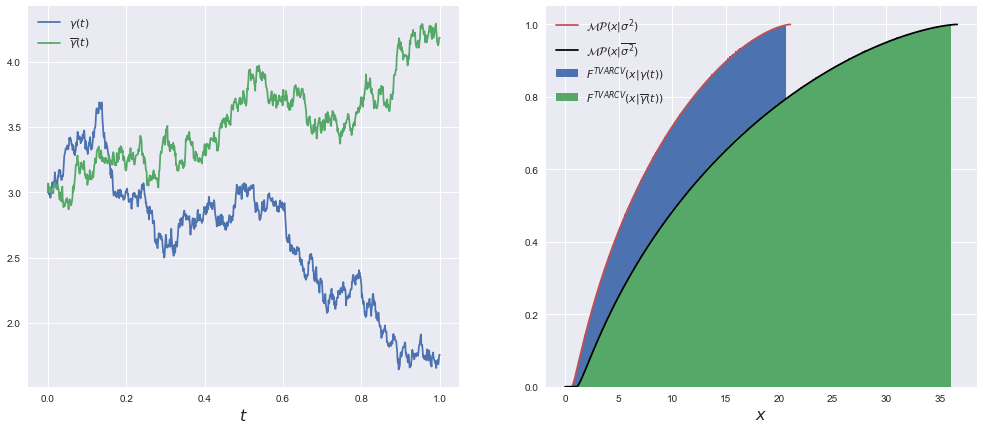
\includegraphics[scale=0.4]{XCIR}
    		\caption{$\eta_p = p, y = 1, \alpha = 5, \beta = 1, \gamma(0) = 3, \xi = 2$}
    		\smallskip
    		\small
    		Left panel shows two different realizations of $\gamma(t)$. On the right panel blue and green histograms are ESD of $\widehat{\Sigma}_p$ for corresponding volatility processes, red and black curve -- Marchenko-Pastur law for different realizations of $\sigma^2$. We see that even with the same parameters of volatility model, we have the different scale parameter in asymptotic spectral distribution for different realizations.
    	\end{center}
    \end{figure}
    		
    \begin{exmp}
    	Let $Y_1, Y_2, \dots$ be i.i.d. random variables $\sim \mathcal{N}(0, 1)$. Let also 
    	\[ \mathbf{N}(t) = (N_1(t), \dots, N_p(t))^T \]
    	be a vector of independent Poisson processes all with intensity $\lambda$ and
    	\[d\mathbf{X}(t) = d\mathbf{W}(t) + \mathbf{Q}(t),  \]
    	where $\mathbf{Q}(t) = (Q_1(t), \dots, Q_p(t))^T $ is a vector of compound Poisson processes, whose components are
    	\[ Q_j(t) = \sum_{i=1}^{N_j(t)} Y_i \quad \forall 1 \leq j \leq p. \]
    	Note, that $Q_j(t)$ are martingales. \\
    	Let us first be in a setting $\lambda = 1$. Then we can see on a figure that both RCV and TVARCV fail. \\
    	However, if we set $\lambda \rightarrow 0$, jumps will happen too frequently and $\mathbf{Q}(t)$ will converge to the simple diffusion process. Due to normality of $Y_i$ in this example, we get
    	\[d\mathbf{Q}(t) \simeq \frac{1}{\sqrt{dt}} d\overline{\mathbf{W}}(t),  \]
    	where $\overline{\mathbf{W}}(t)$ is a $p$-dimensional standard Brownian motion. Then, roughly speaking,
    	\[ \Sigma_p \simeq n \mathbb{I}_{p \times p}. \]
    \end{exmp}
    
    
    \begin{figure}[ht]
    	\begin{center} \centering
    		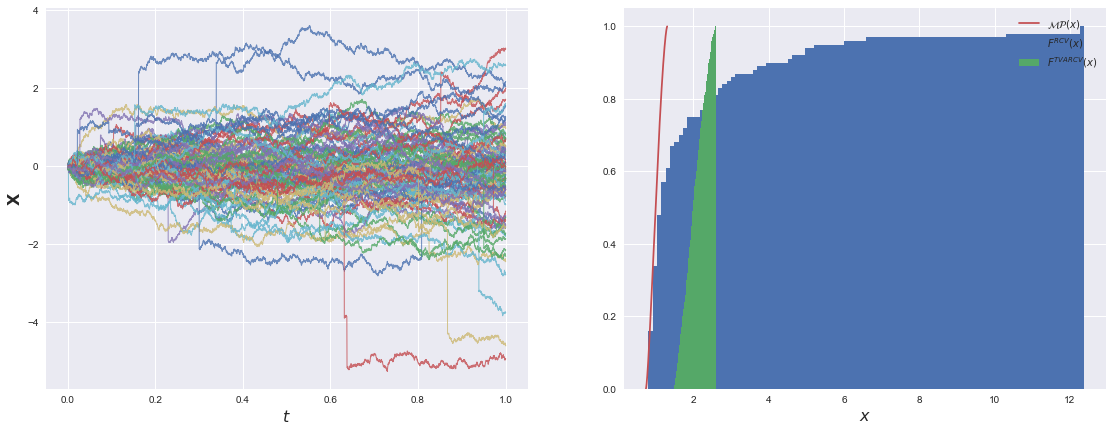
\includegraphics[scale=0.4]{Xjumps}
    		\caption{$n = 5000$, $p = 100$, $\lambda = 1$, $Y_1 \sim \mathcal{N}(0, 1)$}
    		\smallskip
    		\small
    		Jump-diffusion process with jumps, based on compound Poisson process.
    	\end{center}
    \end{figure}
    
    \begin{figure}
       	\begin{center} \centering
       		\includegraphics[scale=0.4]{XCompound}
       		\caption{$n = 1000$, $p = 500$, $\lambda = 10000$, $Y_1 \sim \mathcal{N}(0, 1)$}
       		\smallskip
       		\small
       		We observe that jump-diffusion process converges to pure-diffusion process.
       	\end{center}
       	\begin{center} \centering
       		\includegraphics[scale=0.4]{XCompounduni}
       		\caption{$n = 1000$, $p = 500$, $\lambda = 10000$, $Y_1 \sim \mathcal{U}(0, 1)$}
       		\smallskip
       		\small
       		Jump-diffusion process still converges to pure diffusion process due to Central Limit Theorem, as long as the variance of $Y_i$ is finite.
       	\end{center}
    \end{figure}
    
    \begin{rmrk}
    	For TVARCV to converge to Marchenko-Pastur law, it is sufficient, but not necessary, that $\mathbf{X}(t)$ belongs to the class $\mathcal{C}$. It is noteworthy to show that there can be the case when we have convergence even for RCV.
    \end{rmrk}
    \begin{exmp} \label{counter exmpl}
    	Let drift process be as usual $\boldsymbol{\mu}(t) \equiv 0$ and $\Theta(t)$ be diagonal matrix, which elements are:
    	\[ \Big(\Theta(t)\Big)_{jj} = \sin(\pi t) \mathbf{1}_{\{j \leq p/2\}} + \cos(\pi t) \mathbf{1}_{\{j > p/2\}}, \quad 1 \leq j \leq p.  \]
    	In other words, first $p/2$ elements of the diagonal of $\Theta(t)$ are $\cos(\pi t)$ and the others are $\sin(\pi t)$. It is obvious, that $\mathbf{X}(t)$ doesn't belong to the class $\mathcal{C}$. The ICV matrix is in this case
    	\[ \Sigma_p = \begin{pmatrix}
    	\int_{0}^{1} \cos(\pi t)^2 dt & \cdots & 0 \\
    	\vdots & \ddots & \vdots \\
    	0 & \cdots & \int_{0}^{1} \sin(\pi t)^2 dt
    	\end{pmatrix} 
    	= \frac{1}{2} \mathbb{I}_{p \times p}. \]
    	WHAT DO WE SEEE?
    \end{exmp}
    
    \begin{figure}
    	\begin{center} \centering
    		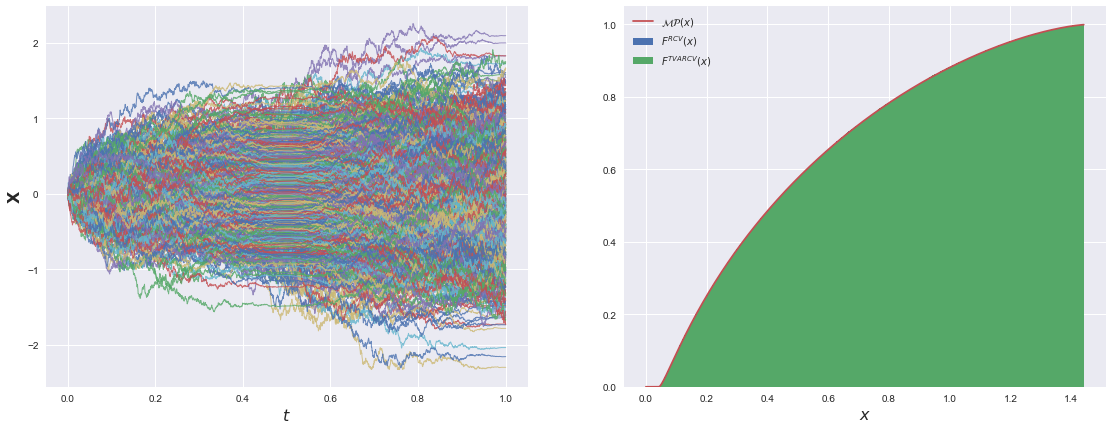
\includegraphics[scale=0.4]{counter}
    		\caption{ $\mathbf{X}(t)$ from Example \ref{counter exmpl}, $n = 3000$, $p=1000$ }
    		\smallskip
    		\small
    		Blue and green histograms coincide with each other and Marchenko-Pastur law.
    	\end{center}
    	\begin{center} \centering
    		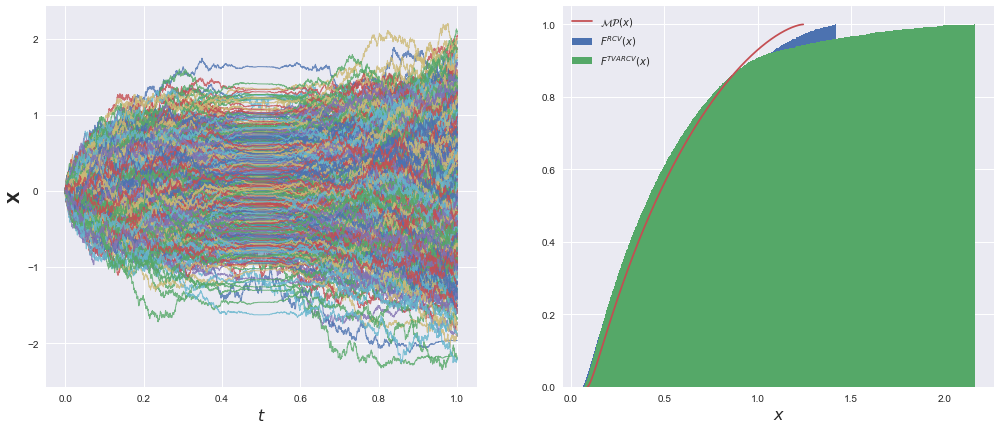
\includegraphics[scale=0.4]{counter2}
    		\caption{ $\mathbf{X}(t)$ from Example \ref{counter exmpl2}, $n = 3000$, $p=1000$ }
    		\smallskip
    		\small
    		TVARCV and RCV give different results, which are both distinct from Marchenko-Pastur law.
    	\end{center}
    \end{figure}
    
    \begin{exmp} \label{counter exmpl2}
    	Let us change slightly the structure of $\Theta(t)$:
    	\[ \Big(\Theta(t)\Big)_{jj} = \sin(\pi t) \mathbf{1}_{\{j \leq p/4\}} + \cos(\pi t) \mathbf{1}_{\{j > p/4\}}, \quad 1 \leq j \leq p.\]
    	The ICV matrix $\Sigma_p$ remains the same. But we can observe from Figure 6.9 that both estimators RCV and TVARCV do not converge to Marchenko-Pastur law anymore. Note, however, that if we fill diagonals $\Theta(t)$ with only $\cos(\pi t)$ or $\sin(\pi t)$, then $\mathbf{X}(t)$ belongs to class $\mathcal{C}$ and TVARCV (but not RCV) converges to $\mathcal{MP}(y, \sigma^2)$.
    \end{exmp}
    
    \appendix
    \chapter{Distribution function for Marchenko-Pastur law}
    	First let us consider the case $0 < y < 1$. Then the domain of the density $f(x)$ is the interval $[a, b]$ and hence $F(x) = 0$ for $ x < a$ and $F(x) = 1$ for $x \geq b$. Inside the interval the formula is
    	\[ 
    	\begin{aligned}
    	F(x) = & \frac{1}{2 \pi y} \Bigg( \pi y +\sqrt{ -x^2-(-1+y)^2 + 2x(1+y)} -\\
    	& (1+y) \arctan\bigg( \frac{1-x+y}{\sqrt{4y - (1-x+y)^2 }} \bigg) + \\
    	& (-1+y) \arctan\bigg( \frac{(-1+y)^2-x(1+y)}{(-1+y)\sqrt{4y - (1-x+y)^2 }} \bigg)  \Bigg).
    	\end{aligned}  \]
    	For $y \geq 1$ we have $f(0) = (1-1/y) \cdot \delta_0(0) $. Therefore, $F(x) = 0$ for $x < 0$, $F(x) = 1 - 1/y$ for $0 \leq x < a$ and $F(x) = 1$ for $x \geq b$. For $x \in [a, b)$ we have:
    	\[ 
    	\begin{aligned}
    	F(x) = & 1 - \frac{1}{2 \pi y} \Bigg( \pi  +\sqrt{4y - (1-x+y)^2 } -\\
    	& (1+y) \arctan\bigg( \frac{1-x+y}{\sqrt{4y - (1-x+y)^2 }} \bigg) + \\
    	& (-1+y) \arctan\bigg( \frac{-(-1+y)^2+x(1+y)}{(-1+y)\sqrt{4y - (1-x+y)^2 }} \bigg)  \Bigg).
    	\end{aligned}  \]
    	
    	\chapter{Python code}
    	\begin{python}
import seaborn as sns
import matplotlib.pyplot as plt
import matplotlib
import numpy as np  
  		
    		
# Marchenko-Pastur probability density function
def MPPdf(x, y, sigmaSq):
    if x == 0:
        if y > 1:
            return np.inf
        return 0
    sqrtY = np.sqrt(y)
    a = sigmaSq * (1 - sqrtY) * (1 - sqrtY)
    b = sigmaSq * (1 + sqrtY) * (1 + sqrtY)
    if x < a or x > b:
        return 0
    pdf = np.sqrt((b - x) * (x - a))
    pdf /= (y * x)
    pdf /= (2 * np.pi * sigmaSq)
    return pdf


# Marchenko-Pastur cumulative distribution function
def MPCdf(x, y, sigmaSq):
    # Marchenko-Pastur cdf for y > 1
    def MPCdfLargeRatio(x, y):
        y1 = 1 - x + y
        temp = np.sqrt(4 * y - y1 * y1)
        y1 /= temp
        y1 = (1 + y) * np.arctan(y1)
        y2 = x * (1 + y)
        y2 -= (y - 1) * (y - 1)
        y2 /= (temp * (y - 1))
        y2 = (y - 1) * np.arctan(y2)
        cdf = np.pi - temp + y1 + y2
        cdf /= (2 * np.pi * y)
        return 1 - cdf

    # Marchenko-Pastur cdf for y <= 1
    def MPCdfSmallRatio(x, y):
        y1 = 1 - x + y
        temp = np.sqrt(4 * y - y1 * y1)
        y1 /= temp
        y1 = (1 + y) * np.arctan(y1)
        if y == 1:
            y2 = 0
        else:
            y2 = x * (1 + y)
            y2 -= (y - 1) * (y - 1)
            y2 /= (temp * (1 - y))
            y2 = (y - 1) * np.arctan(y2)
        cdf = np.pi * y + temp - y1 + y2
        cdf /= (2 * np.pi * y)
        return cdf

    x0 = x / sigmaSq
    sqrtY = np.sqrt(y)
    a = (1 - sqrtY) * (1 - sqrtY)
    b = (1 + sqrtY) * (1 + sqrtY)
    if x0 >= b:
        return 1
    if x0 < 0:
        return 0
    if y > 1:
        if x0 <= a:
            return 1 - 1 / y
        return MPCdfLargeRatio(x0, y)
    if x0 <= a:
        return 0
    return MPCdfSmallRatio(x0, y)


# get sorted eigenvalues
def get_sorted_eigvals(Sigma):
    return np.sort(np.linalg.eigvals(Sigma))


# get empirical spectral distribution
def ESD(x, sorted_eig_values):
    numerator = len(sorted_eig_values[sorted_eig_values <= x])
    denominator = len(sorted_eig_values)
    return numerator / denominator


# TVARCV
def TVARCV(dX, Sigma_RCV):
    (p, n) = dX.shape
    Sigma = np.zeros((p, p))
    for l in range(n):
        dX_l = np.matrix(dX[:, l]).transpose()
        norm = np.linalg.norm(dX_l, ord=2)
        Sigma += dX_l.dot(np.transpose(dX_l)) / (norm * norm)
    Sigma *= np.trace(Sigma_RCV) / n
    return Sigma


# RCV
def RCV(dX):
    (p, n) = dX.shape
    Sigma = np.zeros((p, p))
    for l in range(n):
        dX_l = np.matrix(dX[:, l]).transpose()
        Sigma += dX_l.dot(np.transpose(dX_l))
    return Sigma
  

# function to plot stochastic processes in Figure 1.1
def plot_exmp_1():
    n = 10000
    time = np.linspace(0, 1, n)
    mu = np.array([0, 0, 0])
    X = np.zeros((n, 3))
    dt = time[1] - time[0]
    sqrt_dt = np.sqrt(dt)
    dX = np.random.normal(0, sqrt_dt, 3)
    X[1] = X[0] + dX
    for i in range(1, n - 1):
        dW = np.random.normal(0, sqrt_dt, 3)
        Theta = np.identity(3)
        Theta[0][1] = Theta[1][0] = np.cos(np.pi * time[i])
        Theta[0][2] = Theta[2][0] = np.sin(np.pi * time[i])
        dX_l = np.dot(Theta, dW)
        dX_l += mu * dt
        X[i + 1] = X[i] + dX_l
        dX = np.c_[dX, dX_l]

    plt.plot(time, X)
    plt.legend(["$X_1(t)$", "$X_2(t)$", "$X_3(t)$"], fontsize = 16)
    plt.xlabel('$t$', fontsize = 16)
    plt.ylabel('$\mathbf{X}$', fontsize = 16)
    plt.show()


# function to plot graphs of Marchenko-Pastur law (Figure 2.1)
def plot_MP_law
    y = [0.1, 0.25, 1, 4]
    sigma_sq = [1, 1, 1, 0.3]
    m = 300
    xpdf = np.linspace(1/m, 4, m)
    xcdf = np.linspace(-1/m, 4, m)
    cdf = np.zeros(m)
    pdf = np.zeros(m)
	
    plt.subplot(1, 2, 1)
    for ratio, vol in zip(y, sigma_sq):
        for i in range(m):
    	    pdf[i] = MPPdf(xpdf[i], ratio, vol)
        plt.plot(xpdf, pdf)
    plt.ylim(ymax=2.25)
    # plot infinity line for y > 1
    plt.plot((0, 0), (0, 3), color='C3')
    plt.legend(["$y=0.1, \sigma^2=1$", "$y=0.25, \sigma^2=1$", \
        "$y=1, \sigma^2=1$", "$y=4, \sigma^2=0.3$"])
    plt.xlabel('$x$', fontsize = 16)
    plt.ylabel('$f(x)$', fontsize = 16)
	
    plt.subplot(1, 2, 2)
    for ratio, vol in zip(y, sigma_sq):
        for i in range(m):
            cdf[i] = MPCdf(xcdf[i], ratio, vol)
        plt.plot(xcdf, cdf)
    plt.legend(["$y=0.1, \sigma^2=1$", "$y=0.25, \sigma^2=1$", \
        "$y=1, \sigma^2=1$", "$y=4, \sigma^2=0.3$"]) 
    plt.xlabel('$x$', fontsize = 16)
    plt.ylabel('$F(x)$', fontsize = 16)
	
    plt.show()
    

# function that returns volatility as CIR process
# and corresponding integrated covariance
def get_CIR(t, alpha, beta, xi, x0):
    dt = t[1] - t[0] # we assume times are equally spaced
    exp_mbeta_dt = np.exp(-beta * dt)
    c = 4 * beta / (xi * xi * (1.0 - exp_mbeta_dt))
    degree = 4 * alpha * beta / (xi * xi)
    Y = x0 * np.ones(len(t))
    sigma_sq = alpha * alpha * dt
    for i in range(1, len(gamma)):
        k = c * Y[i - 1] * exp_mbeta_dt
        Y[i] = np.random.noncentral_chisquare(degree, k) / c
        sigma_sq += Y[i] * Y[i] * dt
    return Y, sigma_sq
	    
	    
# function that plots figures for different data
# parameter get_data is a function that accepts parameters n and p
# and returns observed data
def plot_figures(get_data, n, p):
    X, dX, time, sigma_sq = get_data(n, p)
    
    plt.subplot(1, 2, 1)
    plt.plot(time, X, alpha=0.8, linewidth=1)
    plt.xlabel('$t$', fontsize = 16)
    plt.ylabel('$\mathbf{X}$', fontsize = 16)    
    
    plt.subplot(1, 2, 2)
    Sigma_RCV = RCV(dX)
    sorted_eigvals_RCV = get_sorted_eigvals(Sigma_RCV)
    plt.hist(sorted_eigvals_RCV, p, cumulative=True, normed=True)
    
    sorted_eigvals_TVARCV = get_sorted_eigvals(TVARCV(dX, Sigma_RCV))
    plt.hist(sorted_eigvals_TVARCV, p, cumulative=True, normed=True)
    
    cdf_len = 3000
    cdf = np.zeros(cdf_len)
    sqrt_ratio = np.sqrt(p / n)
    a = 1 - sqrt_ratio
    b = 1 + sqrt_ratio
    a *= sigma_sq *a
    b *= sigma_sq * b
    x = np.linspace(a, b, cdf_len)
    for i in range(cdf_len):
        cdf[i] = MPCdf(x[i], p / n, sigma_sq)
    plt.plot(x, cdf)
    
    plt.xlabel('$x$', fontsize = 16)
    plt.legend(['$\mathcal{MP}(x)$', \
                '$F^{RCV}(x)$', '$F^{TVARCV}(x)$'])
    plt.show()
    
    
# function that returns data with non-constant volatility
def get_data_for_volatile_gamma(n, p):
    time = np.zeros(n + 1)
    X = np.zeros((n + 1, p))
    delta_time = 1/n
    dX = 0.03 * np.random.normal(0, np.sqrt(delta_time), p)
    X[1] = X[0] + dX
    time[1] += delta_time
    newSin = 0
    for i in range(1, n):
        delta_time = np.exp(np.mean(X[i, :])) / n
        time[i + 1] = time[i] + delta_time
        dW = np.random.normal(0, np.sqrt(delta_time), p)
        oldSin = newSin
        newSin = np.sin(2 * np.pi * (i + 1) / n)
        dSin = newSin - oldSin
        Gamma = 0.0009 + n * 0.0008 * dSin / (2 * np.pi)
        Gamma = np.sqrt(Gamma)
        dX_l = Gamma * dW
        X[i + 1] = X[i] + dX_l
        dX = np.c_[dX, dX_l]
    return X, dX, time, 0.0009
    

# function that returns data for non-equidistant observation times,
# note that time[n-1] may be not equal to 1 
def get_data_poisson_times(n, p):
    time = np.zeros(n + 1)
    X = np.zeros((n + 1, p))
    rate = 1 / n
    delta_time = np.random.exponential(rate)
    dX = 0.03 * np.random.normal(0, np.sqrt(delta_time), p)
    X[1] = X[0] + dX
    time[1] += delta_time
    newSin = 0
    for i in range(1, n):
        delta_time = np.random.exponential(rate)
        time[i + 1] = min(time[i] + delta_time, 1)
        dW = np.random.normal(0, np.sqrt(delta_time), p)
        oldSin = newSin
        newSin = np.sin(2 * np.pi * time[i+1])
        dSin = newSin - oldSin
        Gamma = 0.0009 + 0.0008 * dSin / (2 * np.pi * delta_time)
        Gamma = np.sqrt(Gamma)
        dX_l = Gamma * dW
        X[i + 1] = X[i] + dX_l
        dX = np.c_[dX, dX_l]
    return X, dX, time, 0.0009
    
    
# function that returns data for cos/sin case 
def get_data_for_cossin(n, p):
    time = np.zeros(n + 1)
    X = np.zeros((n + 1, p))
    delta_time = 1/n
    dW = np.random.normal(0, np.sqrt(delta_time), p)
    Theta = np.identity(p)
    for j in range(0, int(p/2)):
    Theta[j][j] = 0
    dX = np.dot(Theta, dW)
    X[1] = X[0] + dX
    time[1] += delta_time
    for i in range(1, n):
        time[i + 1] = time[i] + delta_time
        dW = np.random.normal(0, np.sqrt(delta_time), p)
        nsin = np.sin(np.pi * (i + 1) / n)
        ncos = np.cos(np.pi * (i + 1) / n)
        Theta = np.identity(p) * ncos
        for j in range(0, int(p/2)):
            Theta[j][j] = nsin
        dX_l = np.dot(Theta, dW)
        X[i + 1] = X[i] + dX_l
        dX = np.c_[dX, dX_l]
return X, dX, time, 0.5    
    

# function that simulates jump-diffusion process
# with volatility 1, compound Poisson process with rate 1
# and jumps with standard normal distribution
def get_data_jumps(n, p):
    X = np.zeros((n + 1, p))
    time = np.linspace(0, 1, n + 1)
    dt = time[1] - time[0]
    gamma = 1
    sqrt_dt = np.sqrt(dt)
    dX = gamma * np.random.normal(0, sqrt_dt, p)
    X[1] = X[0] + dX
    rate = 1
    jump_time = np.random.exponential(1 / rate, p)
    for i in range(1, n):
        dX_l = np.random.normal(0, sqrt_dt, p)
        dX_l *= gamma
        for j in range(p):
            if jump_time[j] <= i / n:
                dX_l[j] += np.random.normal(0, 1)
                jump_time[j] += np.random.exponential(1 / rate)
        X[i + 1] = X[i] + dX_l
        dX = np.c_[dX, dX_l]
    return X, dX, time, gamma


# function that simulates data with gamma as CIR process
# with parameters alpha = 5, beta = 1, xi = 2 and gamma(0) = 3   
def get_data_stochastic_gamma(n, p):
    sqrt_p = np.sqrt(p)
    X = np.zeros((n + 1, p))
    time = np.linspace(0, 1, n + 1)
    dt = time[1] - time[0]
    alpha = 5
    beta = 1
    xi = 2
    gamma0 = 3
    gamma_sq = gamma0 * gamma0
    gamma = gamma0
    sigma_sq = alpha * alpha * dt
    volatility = gamma0 * np.ones(len(time))
    sqrt_dt = np.sqrt(dt)
    dX = gamma * np.random.normal(0, sqrt_dt, p)
    X[1] = X[0] + dX
    for i in range(1, n):
        dX_l = np.random.normal(0, sqrt_dt, p)
        dW = np.sum(dX_l) / sqrt_p
        dg = beta * (alpha - gamma_sq) * dt + xi * gamma * dW
        gamma_sq += dg
        gamma = np.sqrt(gamma_sq)
        sigma_sq += gamma_sq * dt
        volatility[i] = gamma
        dX_l *= gamma
        X[i + 1] = X[i] + dX_l
        dX = np.c_[dX, dX_l]
    return X, dX, time, sigma_sq
    
\end{python}
    	
   	% bibliography, glossary and index would go here.
   	\addcontentsline{toc}{part}{Bibliography}
   	\bibliographystyle{stylefile}
   	\nocite{*}
   	\bibliography{biblio}
   	
   	\newpage
   	\large
   	\textbf{Declaration} \\
   	
   	I hereby declare that I have made the present work independent and without any help whatsoever, and have not used any sources other than those indicated.\\
   	
   	Furthermore, I assure that this work has not yet been presented as a dissertation elsewhere. \\
   	
   	Datum, unterschrift
\end{document}
